\documentclass[a4paper]{article}

%% Language and font encodings
\usepackage[english]{babel}
\usepackage[utf8x]{inputenc}
\usepackage[T1]{fontenc}

\usepackage{tikz}
\usetikzlibrary{matrix}
\usepackage{algpseudocode} 
%\usepackage{standalone}
%% Sets page size and margins
\usepackage[a4paper,top=3cm,bottom=2cm,left=3cm,right=3cm,marginparwidth=1.75cm]{geometry}
\usepackage{amsmath}
\usepackage{amsthm}
\usepackage{amssymb}
\usepackage{pdfpages}

\newtheorem{theorem}{Theorem}
\newtheorem{lemma}[theorem]{Lemma}

\begin{document}
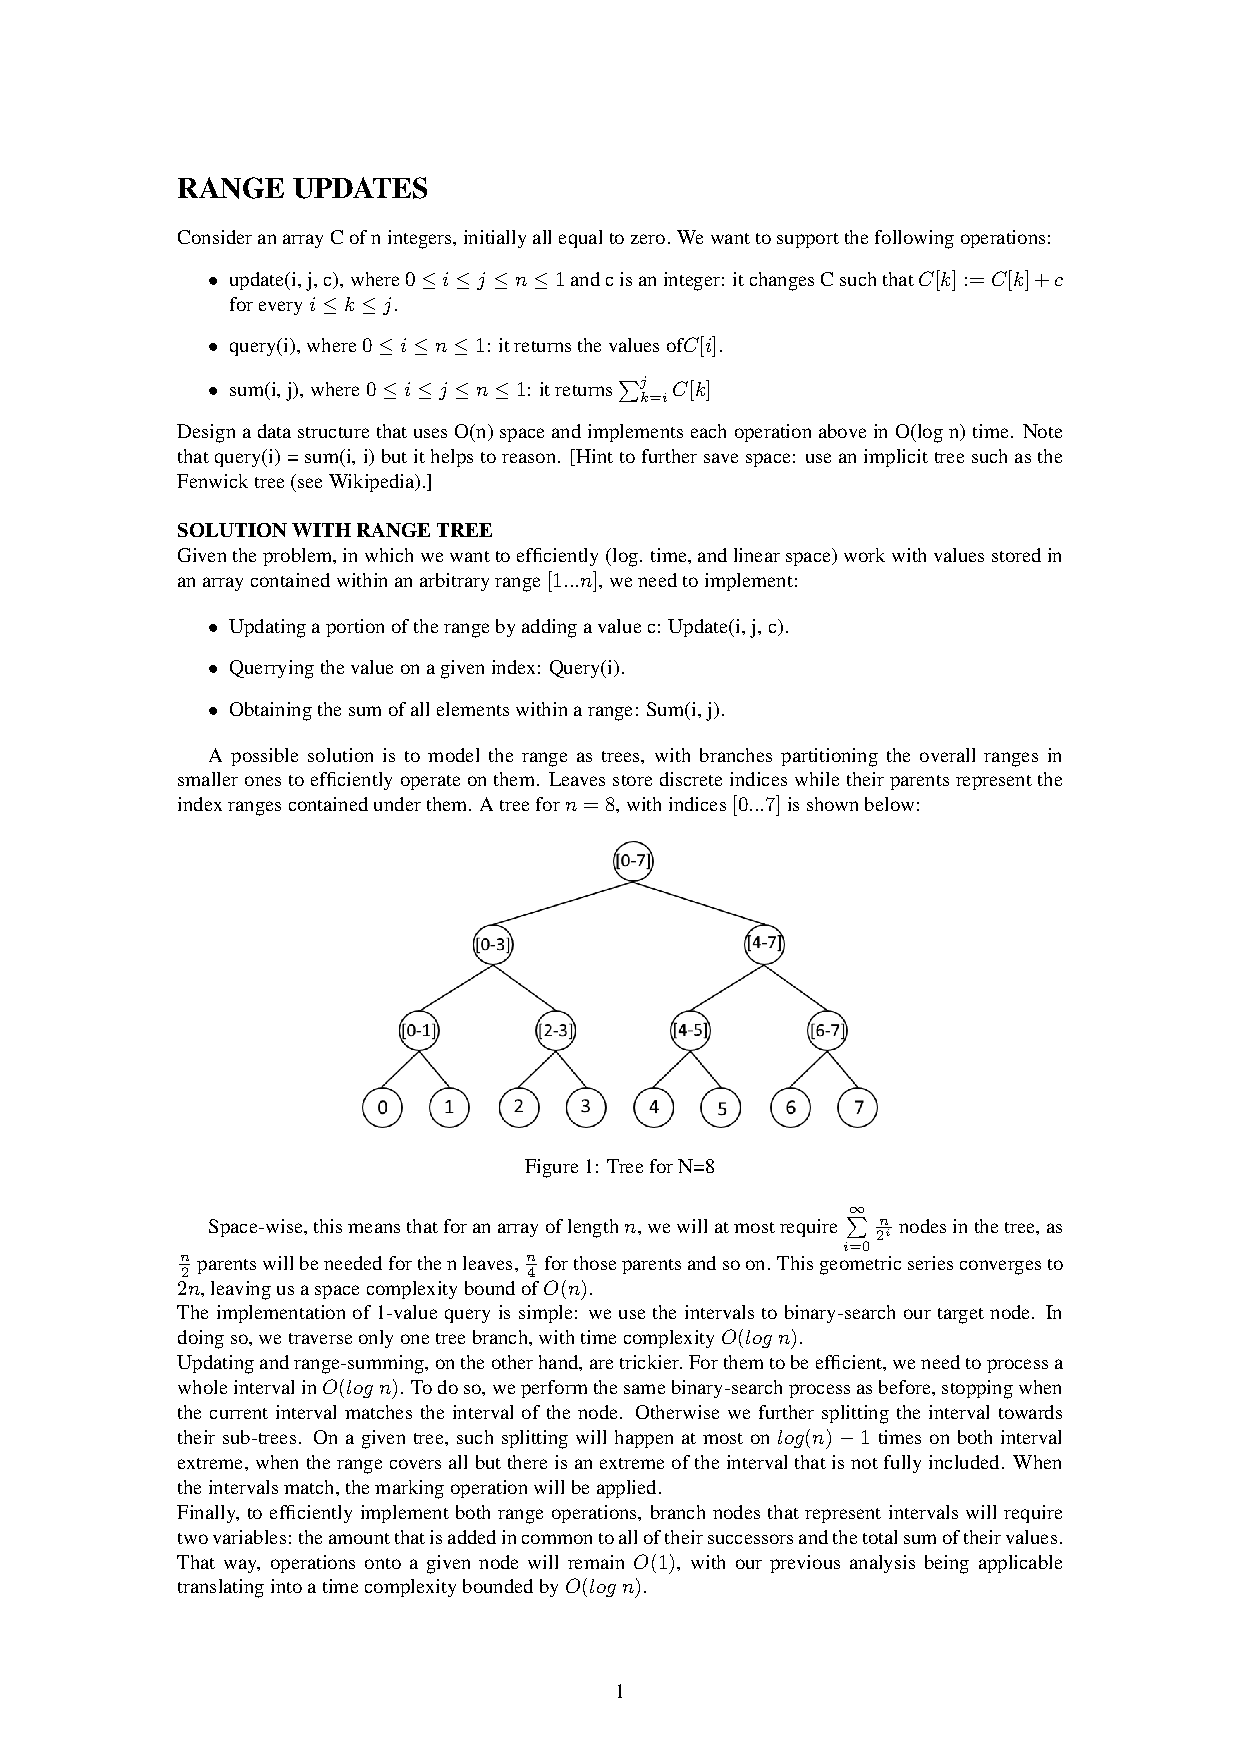
\includepdf[pages={1,2,3,4}]{../EX01/Problem1_SOLUTION}
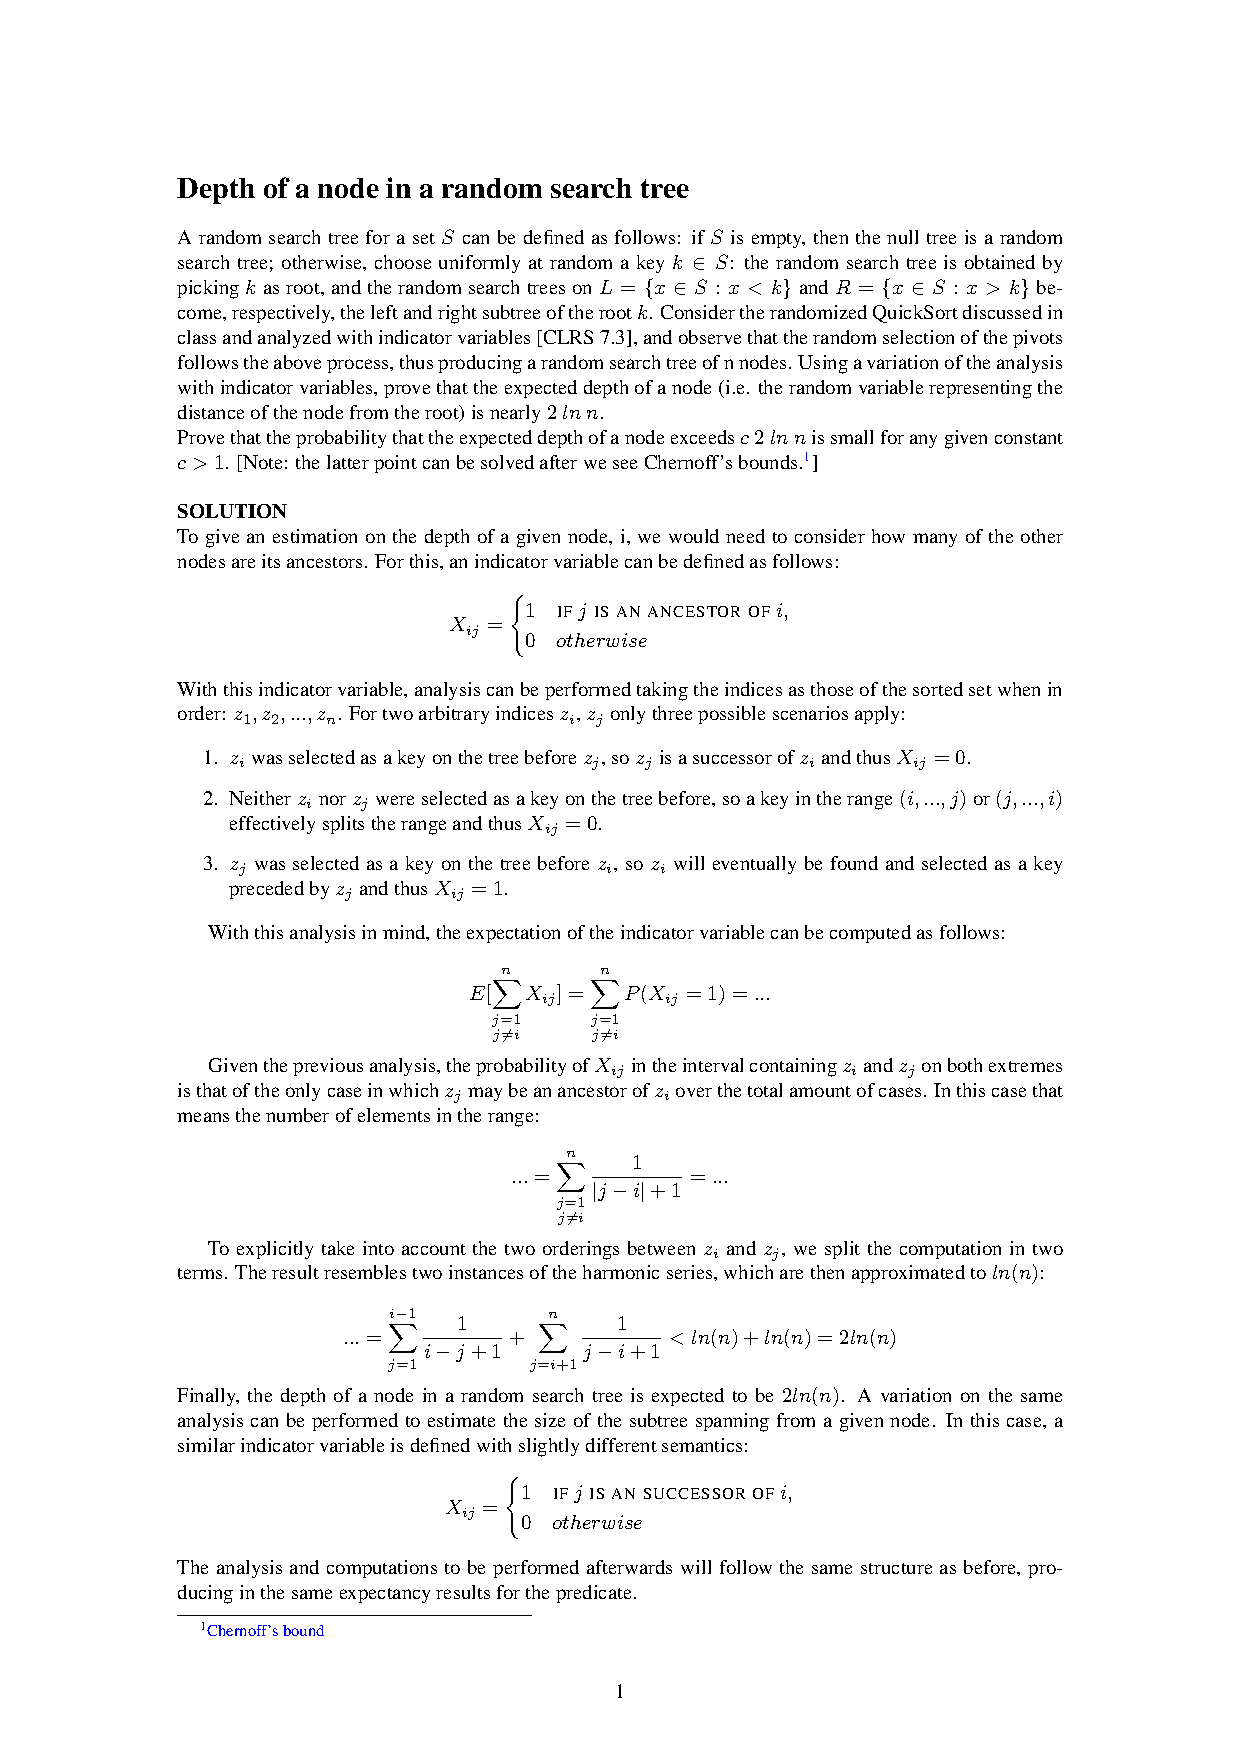
\includepdf[pages={1,2}]{../EX02/Problem2_SOLUTION}
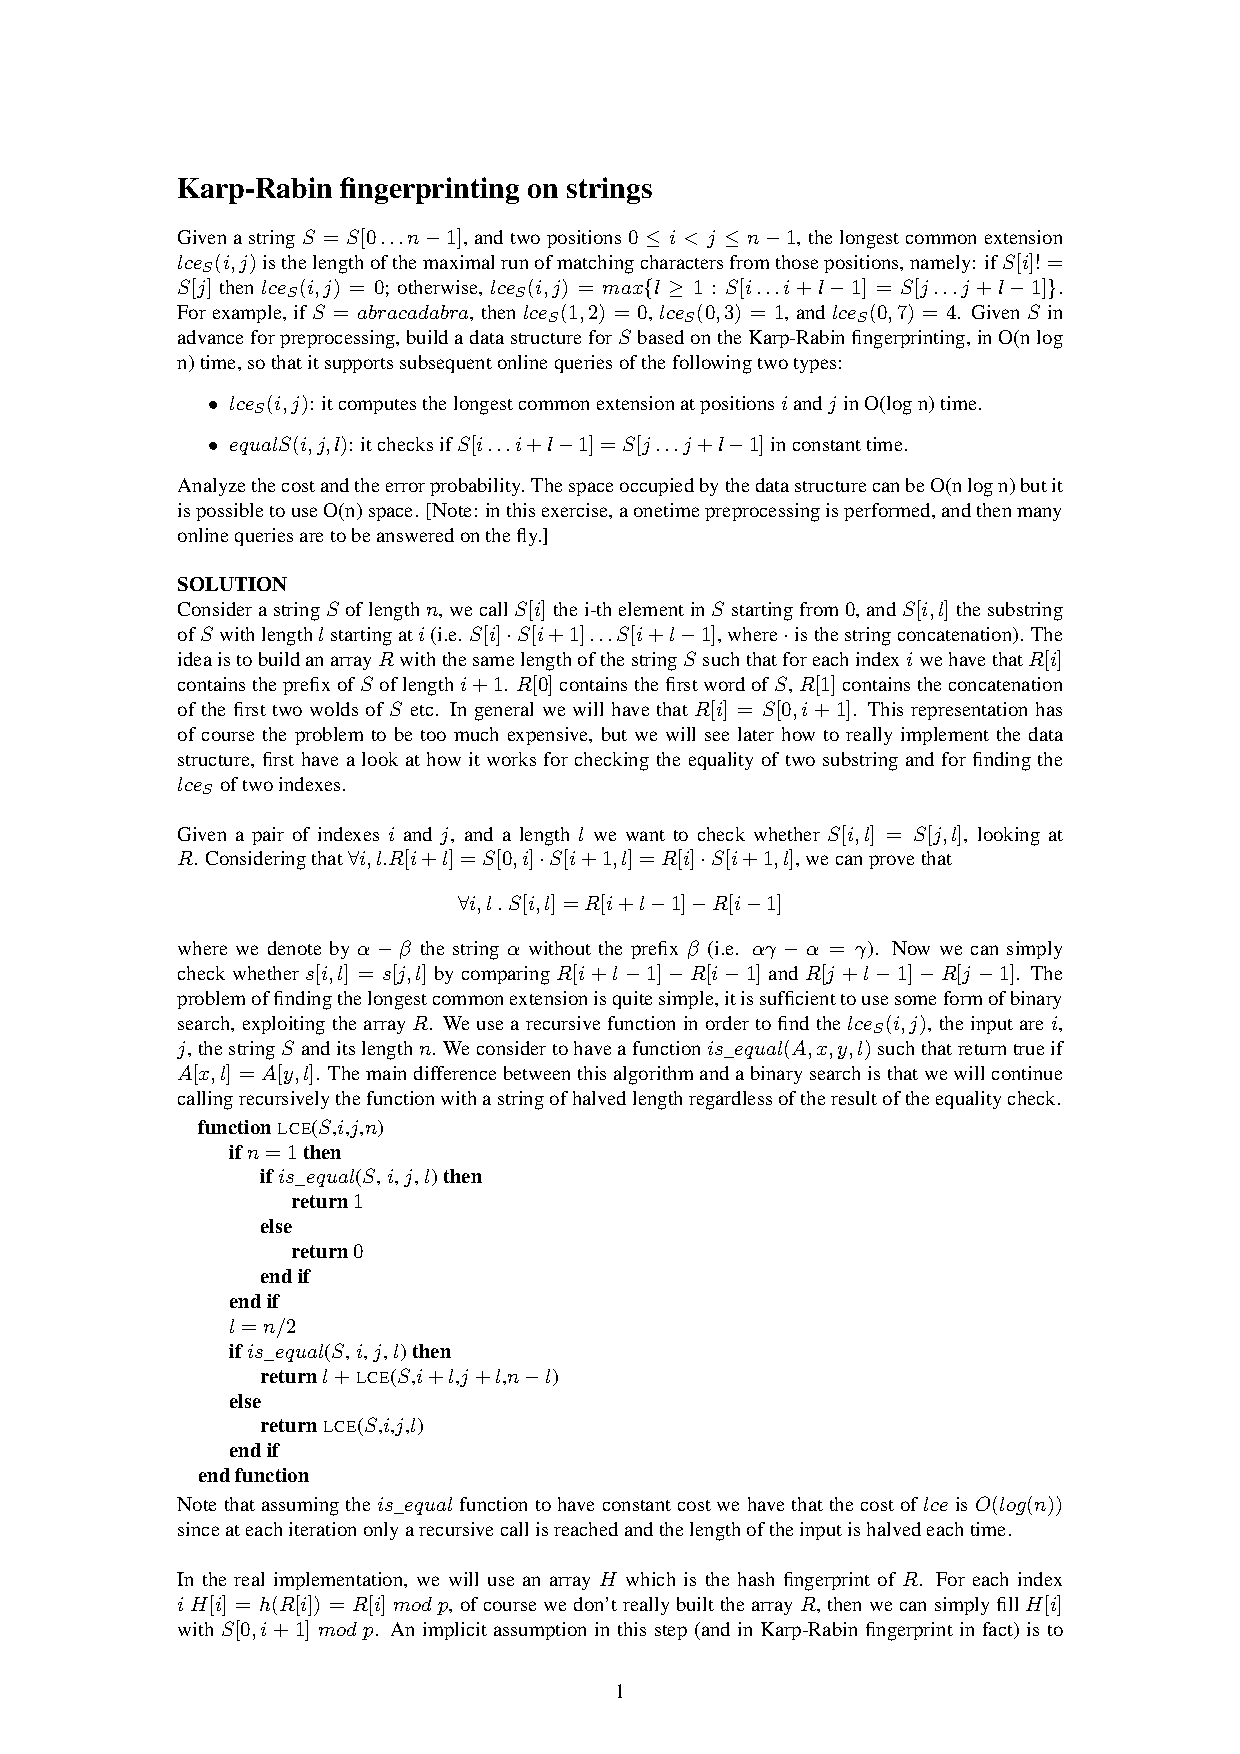
\includepdf[pages={1,2,3}]{../EX03/Problem3_SOLUTION}
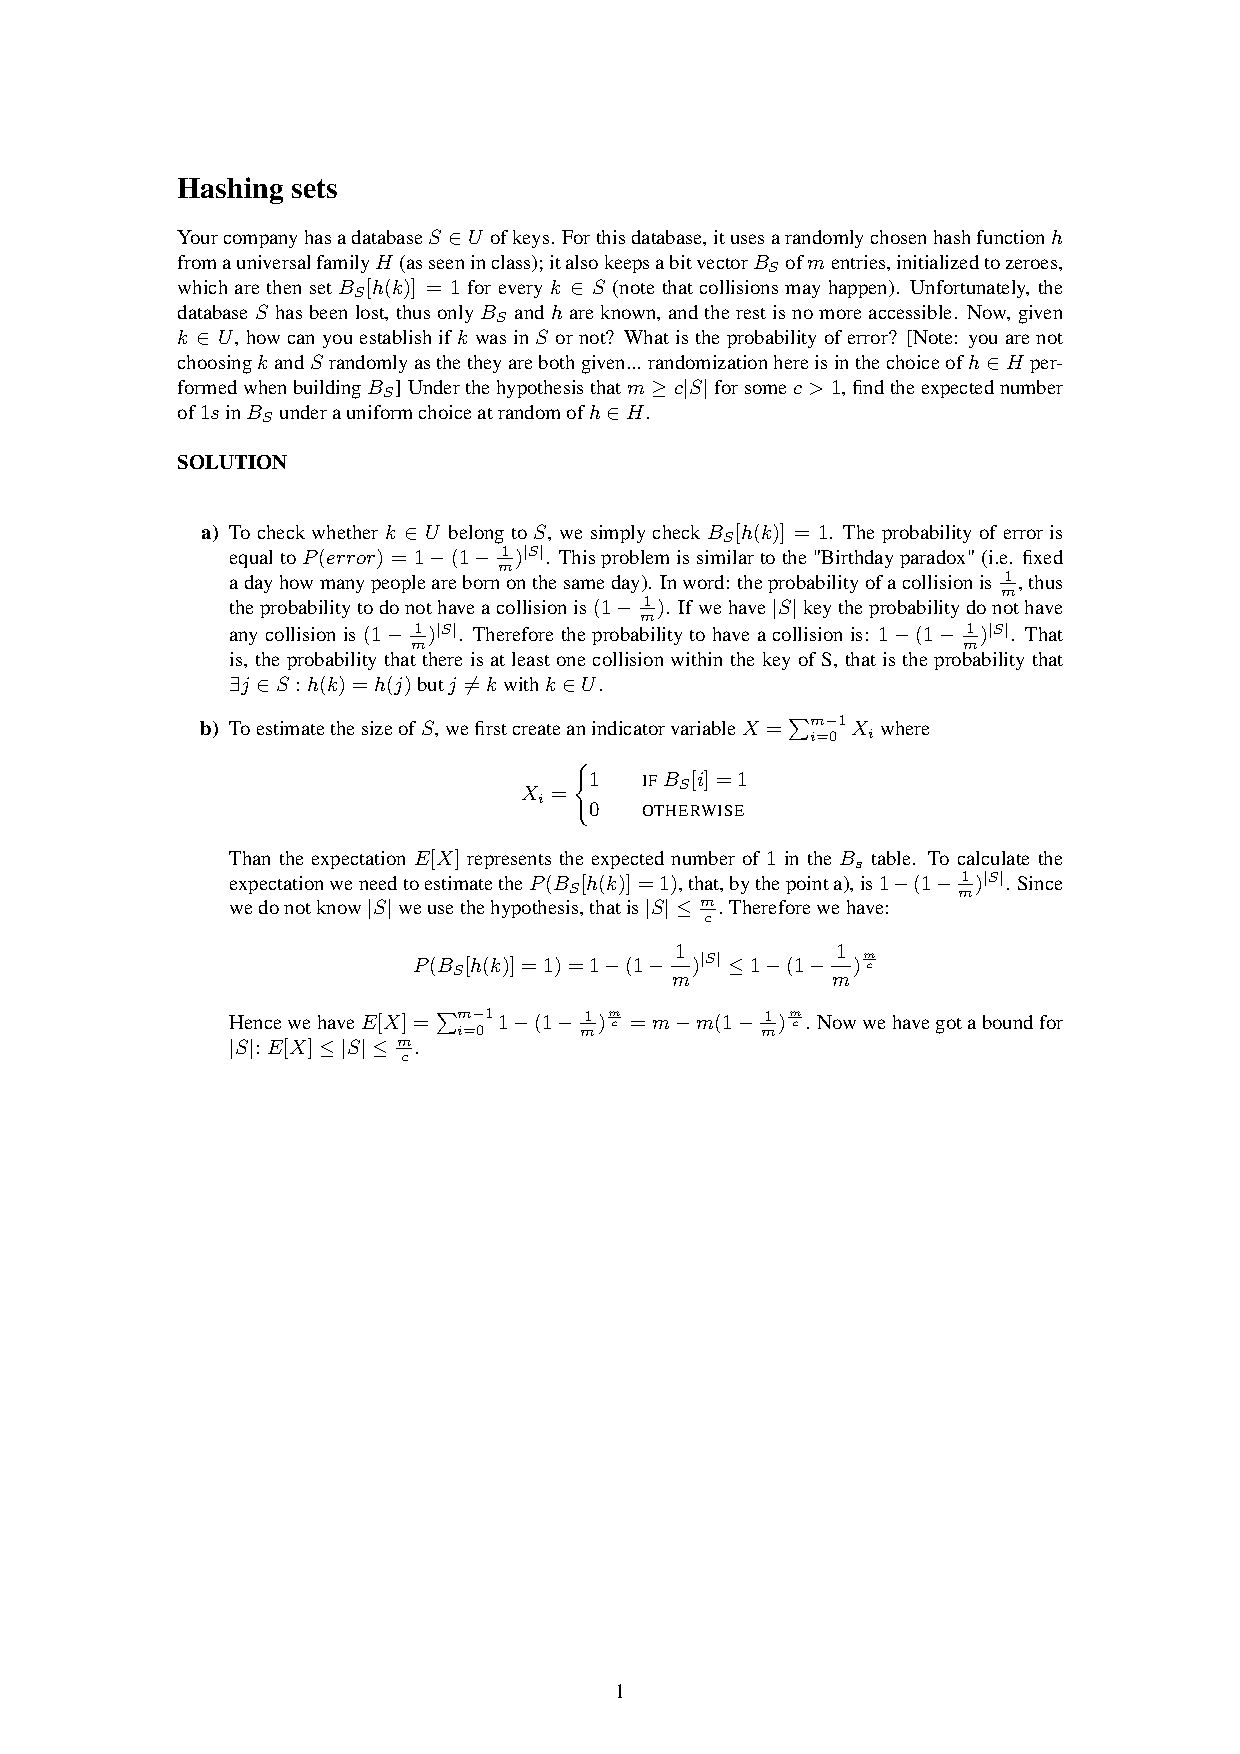
\includepdf[pages={1}]{../EX04/Problem4_SOLUTION}
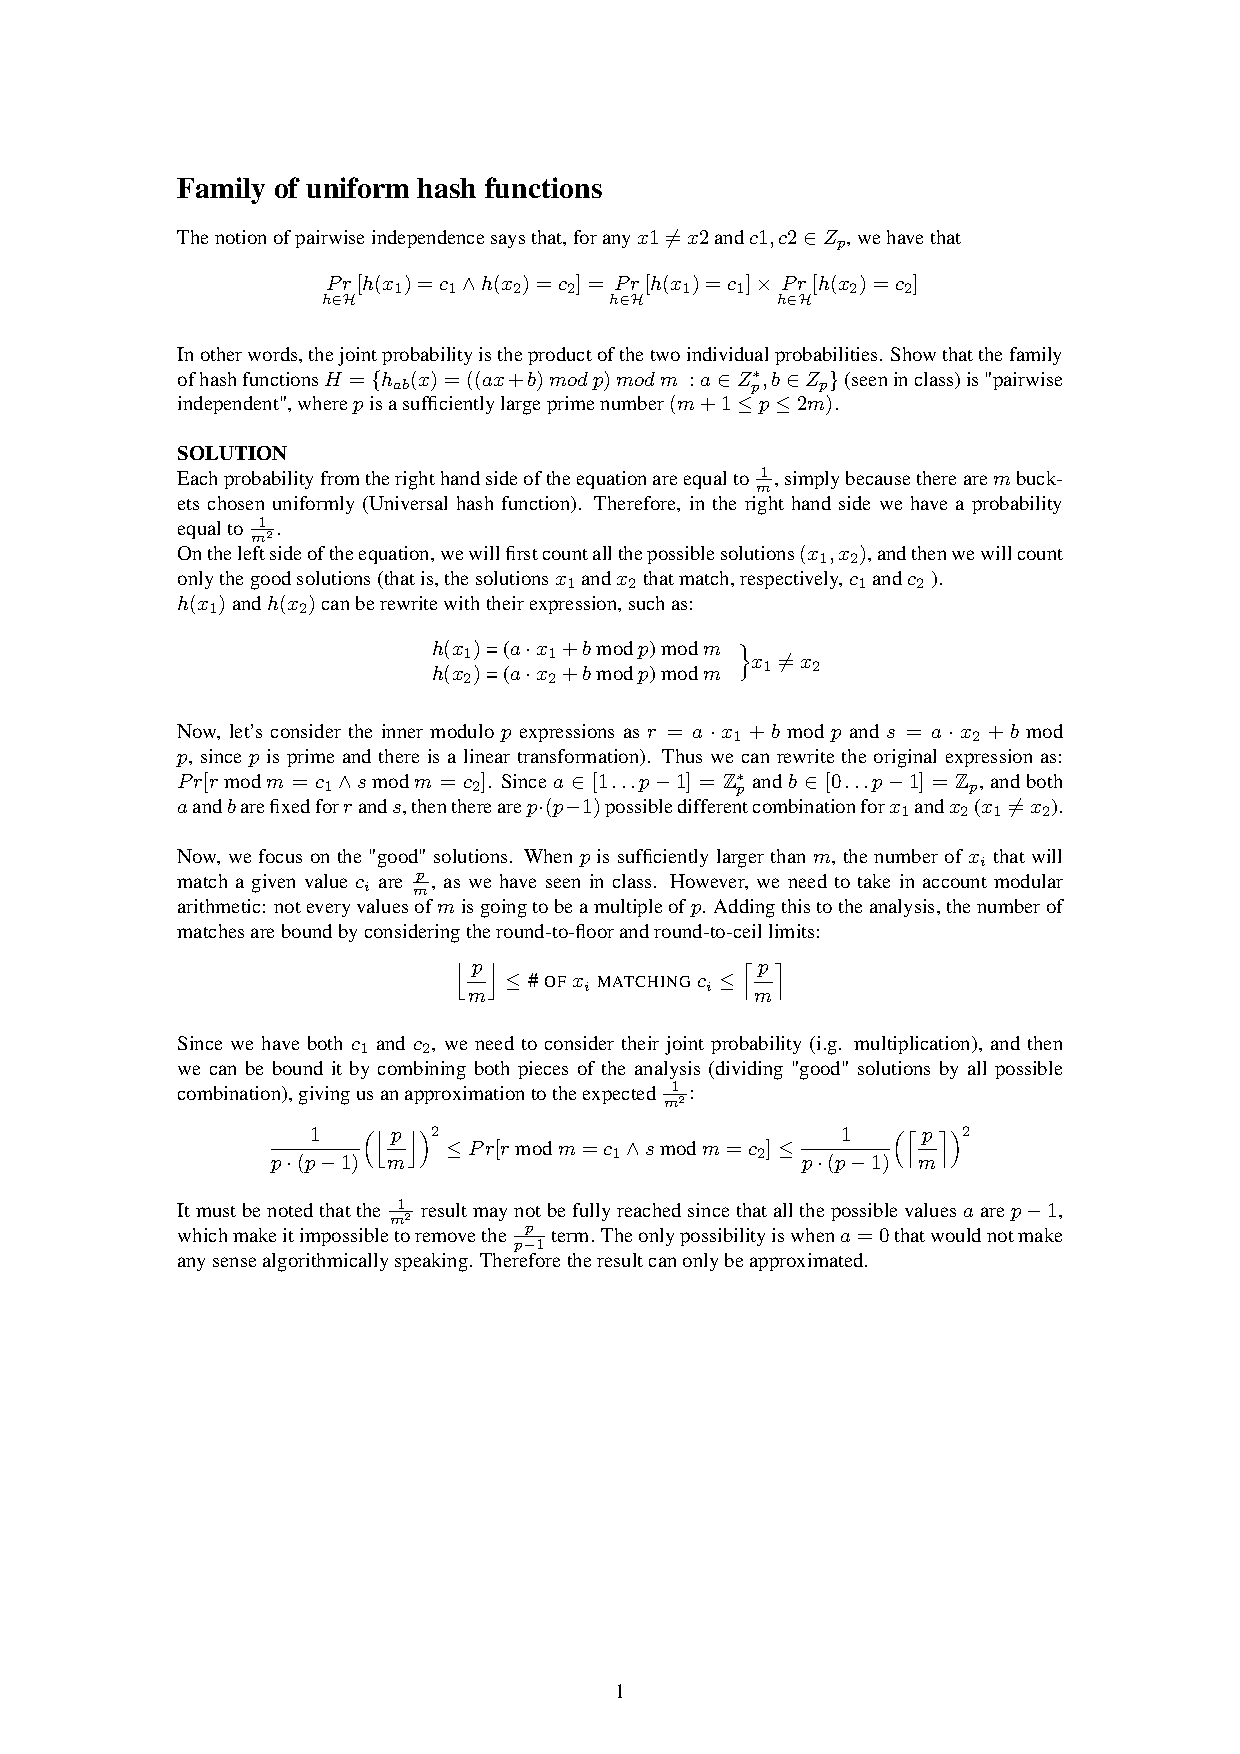
\includepdf[pages={1}]{../EX05/Problem5_SOLUTION}
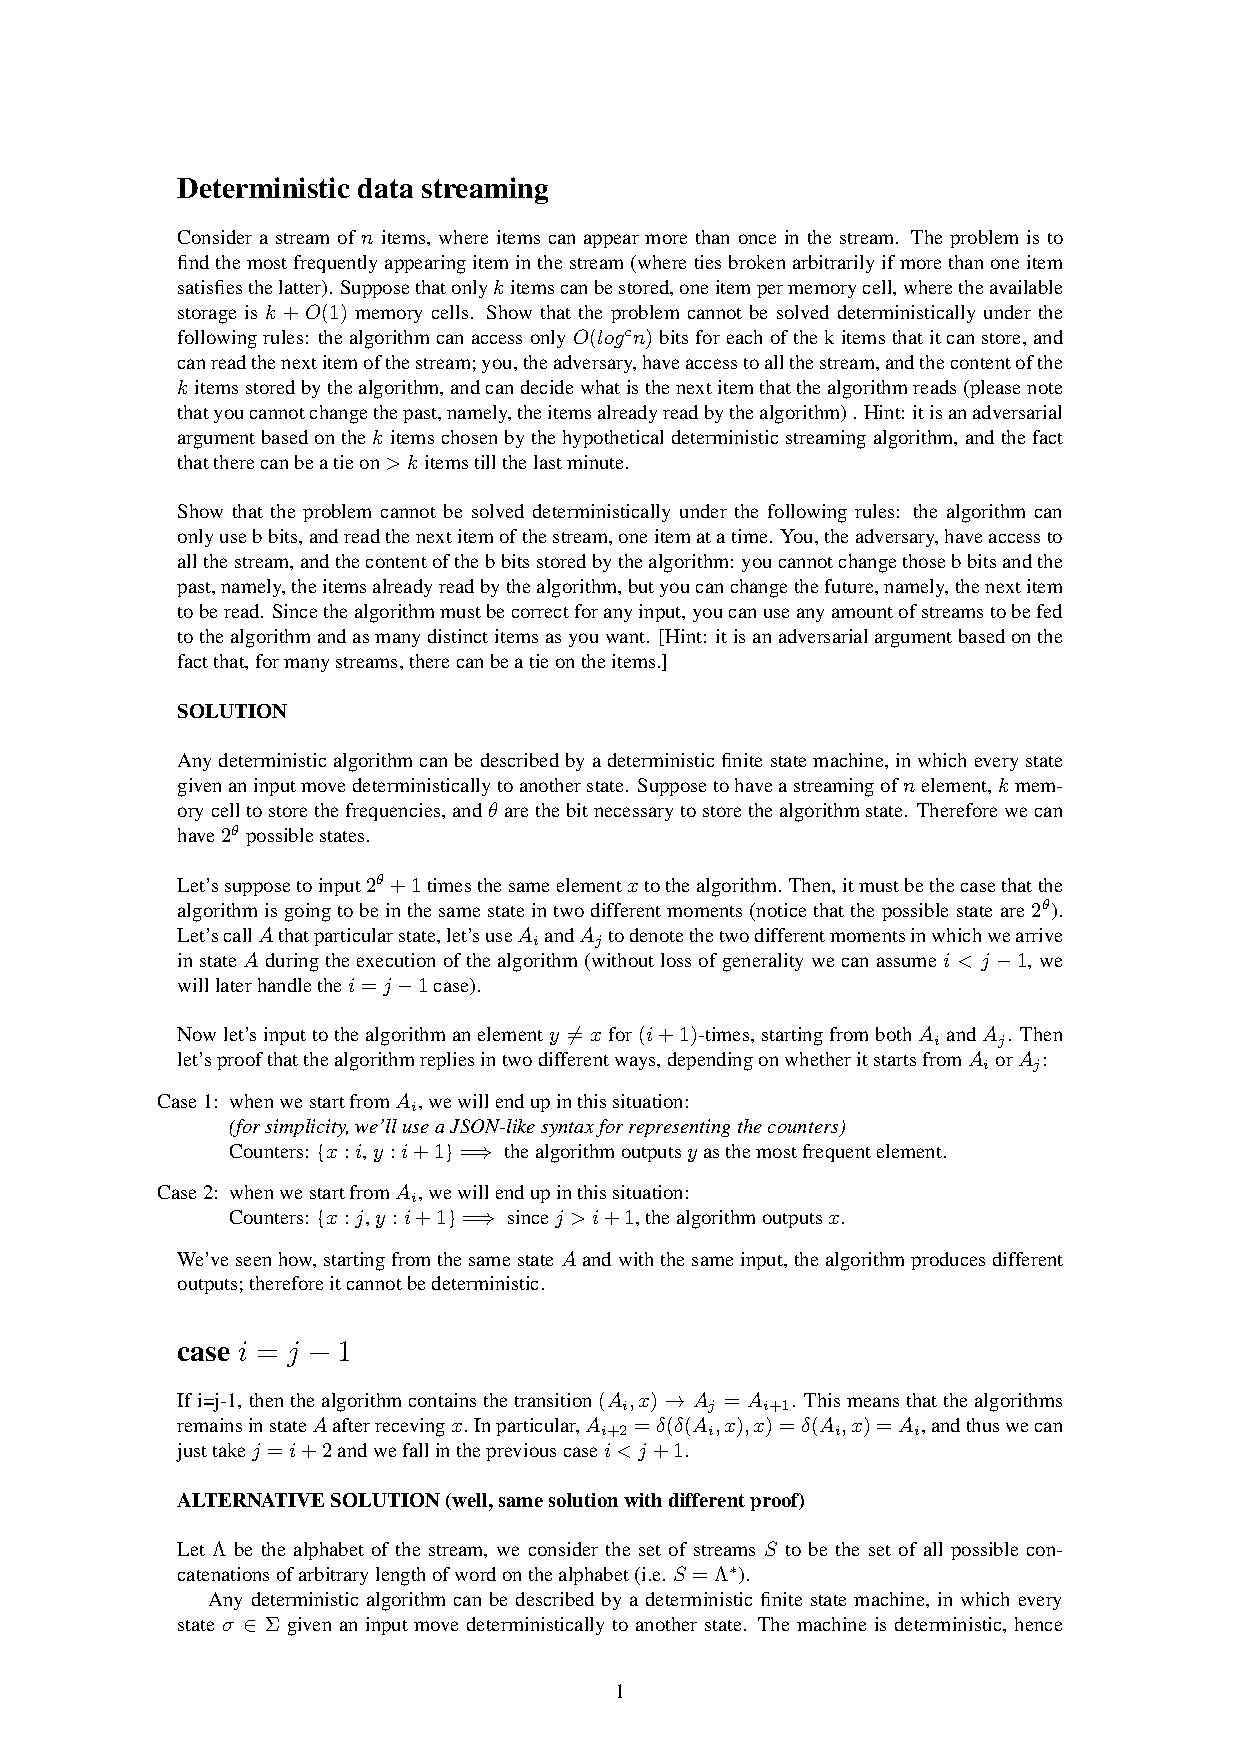
\includepdf[pages={1}]{../EX06/Problem6_SOLUTION}
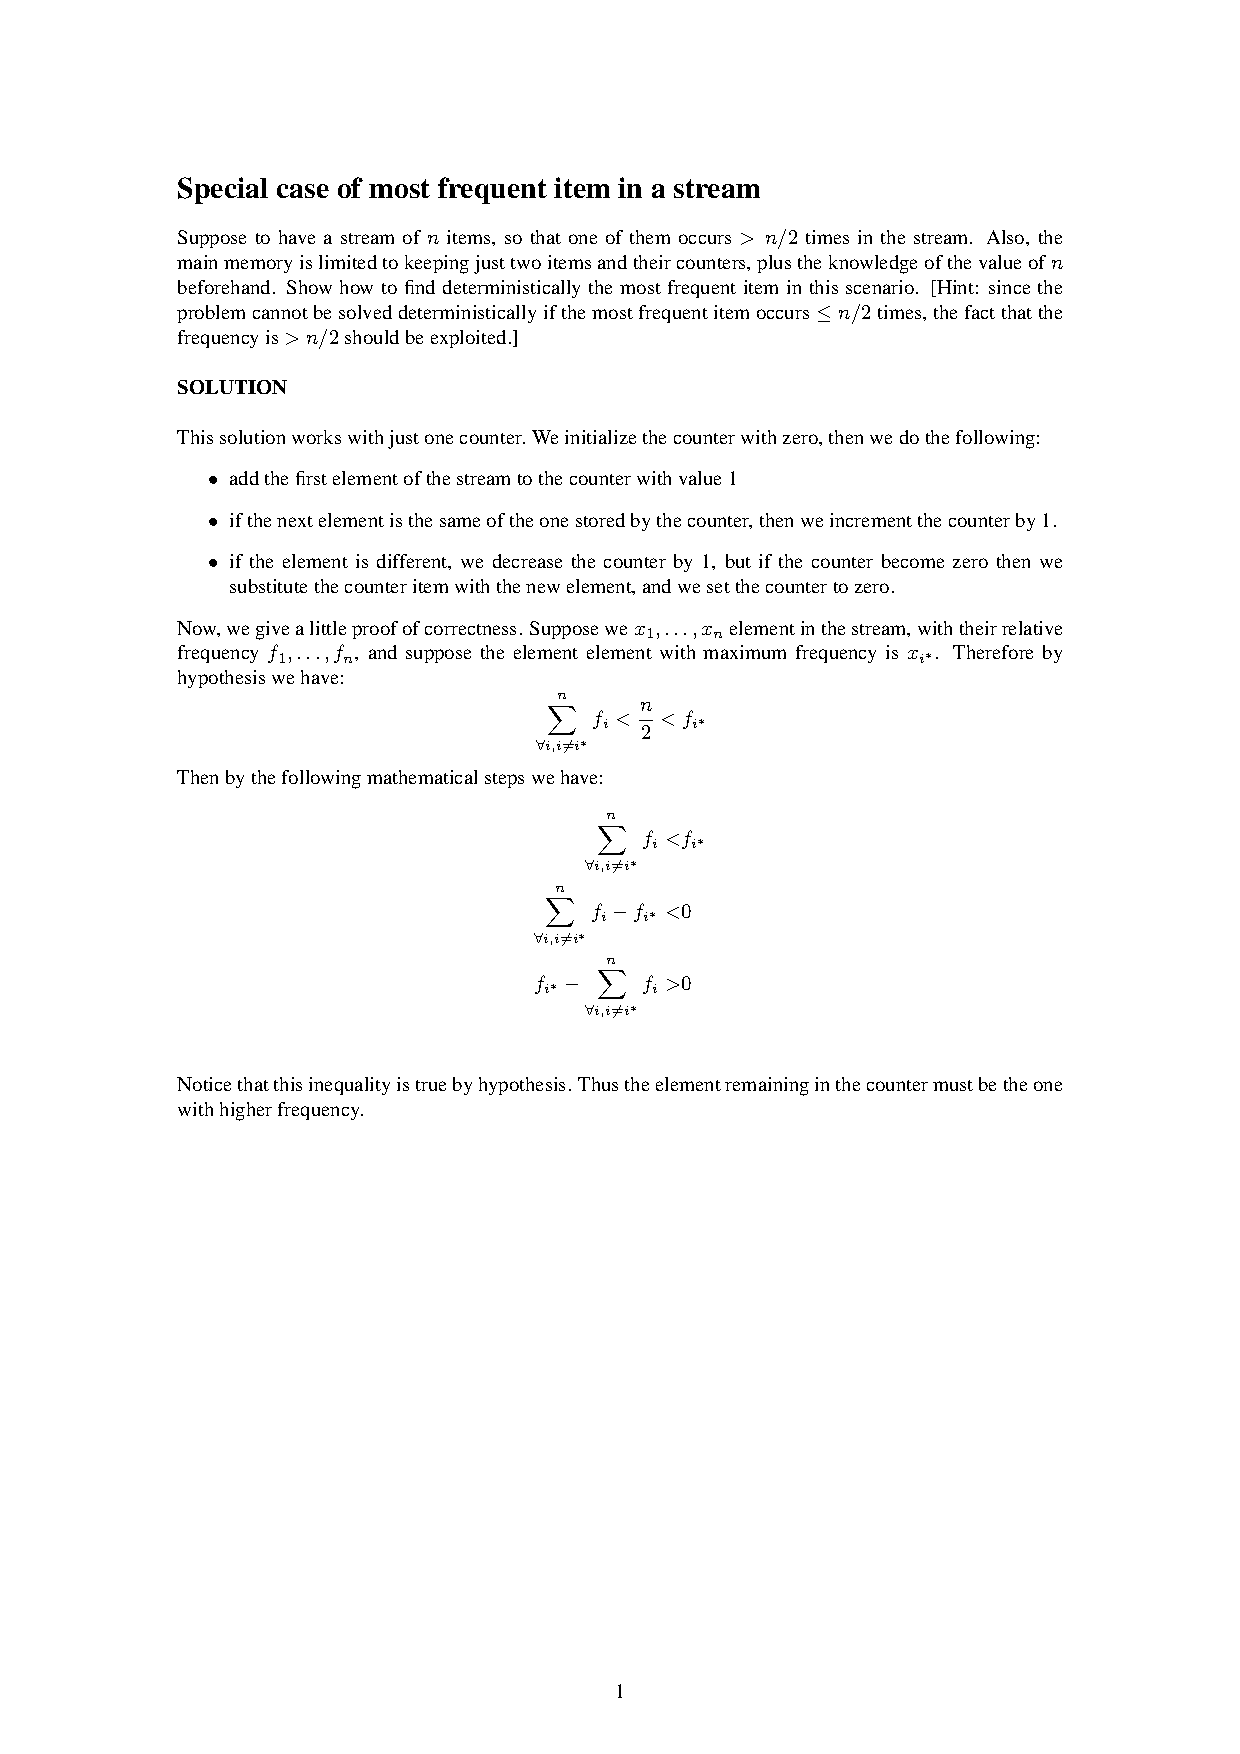
\includepdf[pages={1}]{../EX07/Problem7_SOLUTION}
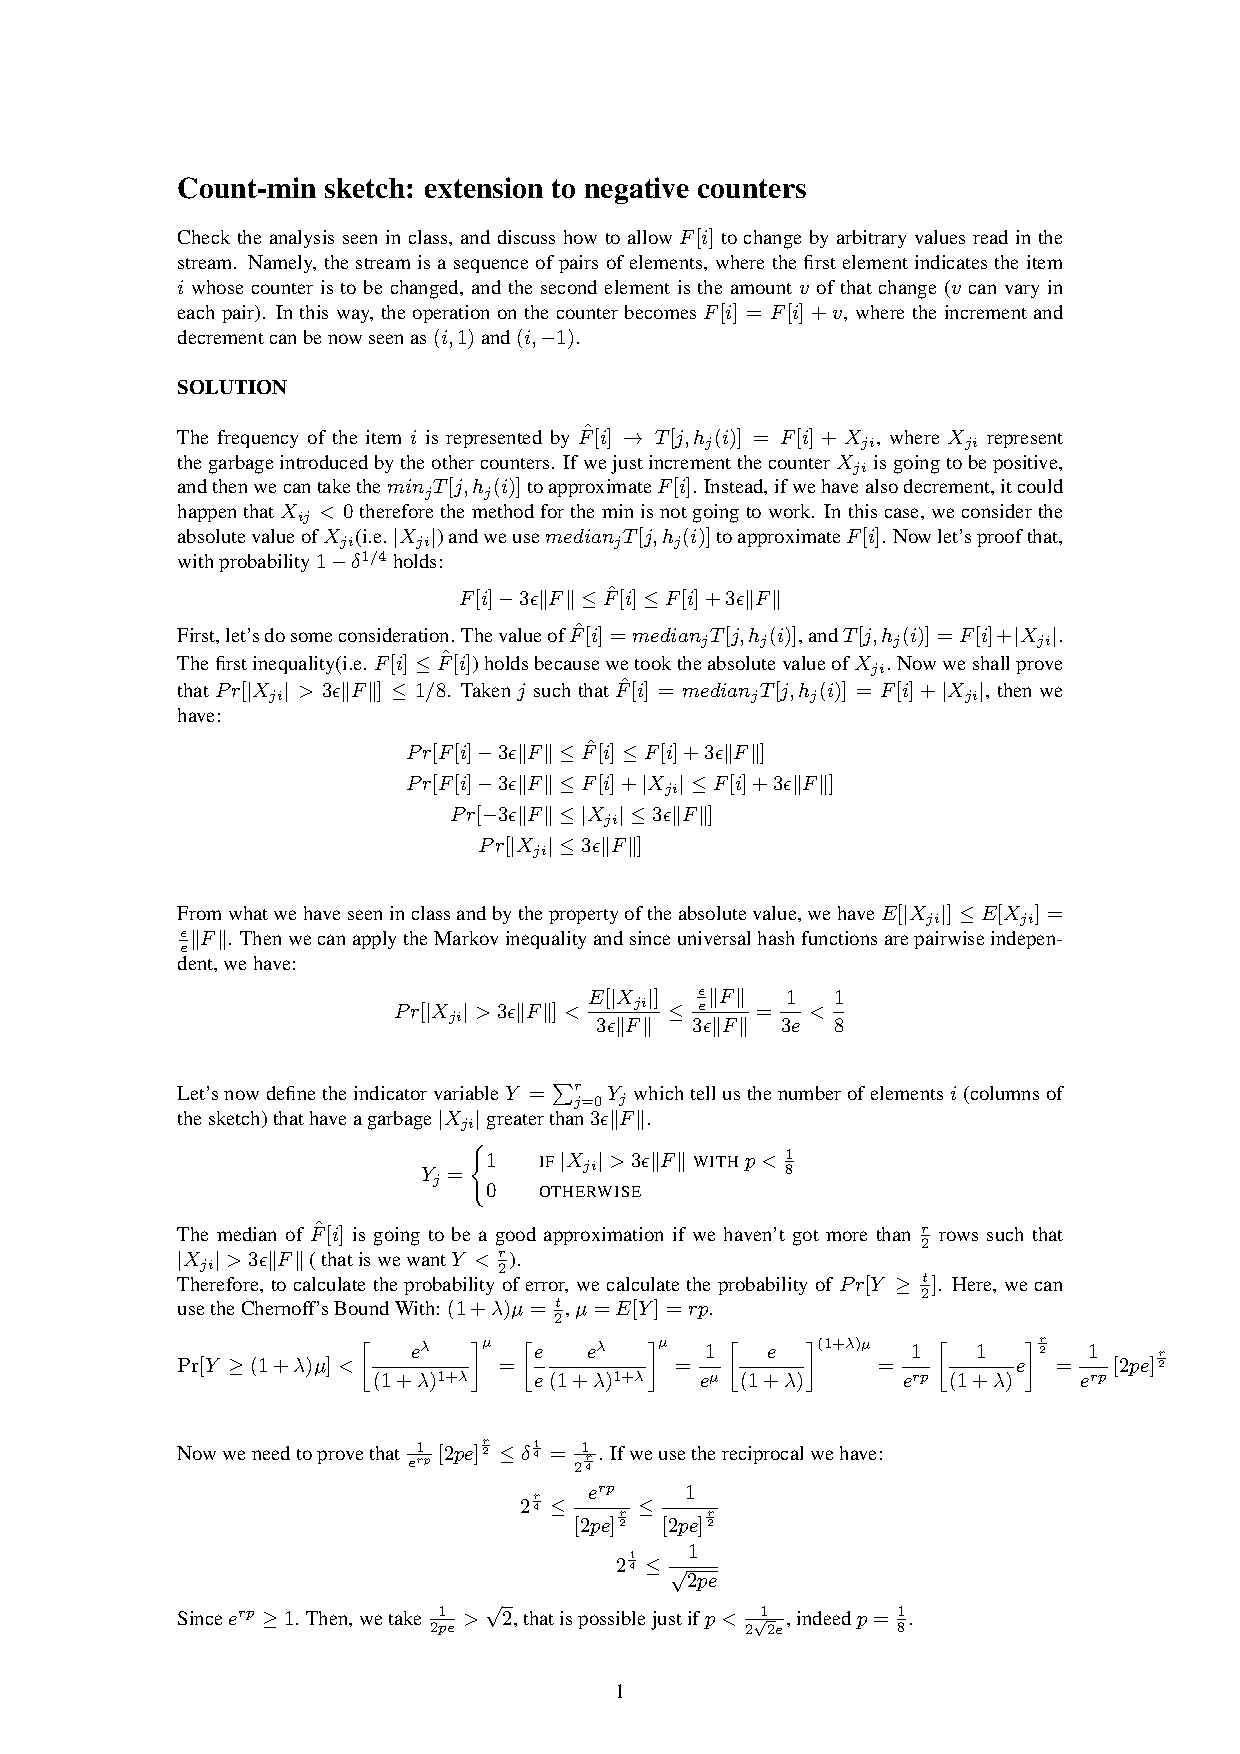
\includepdf[pages={1}]{../EX08/Problem8_SOLUTION}
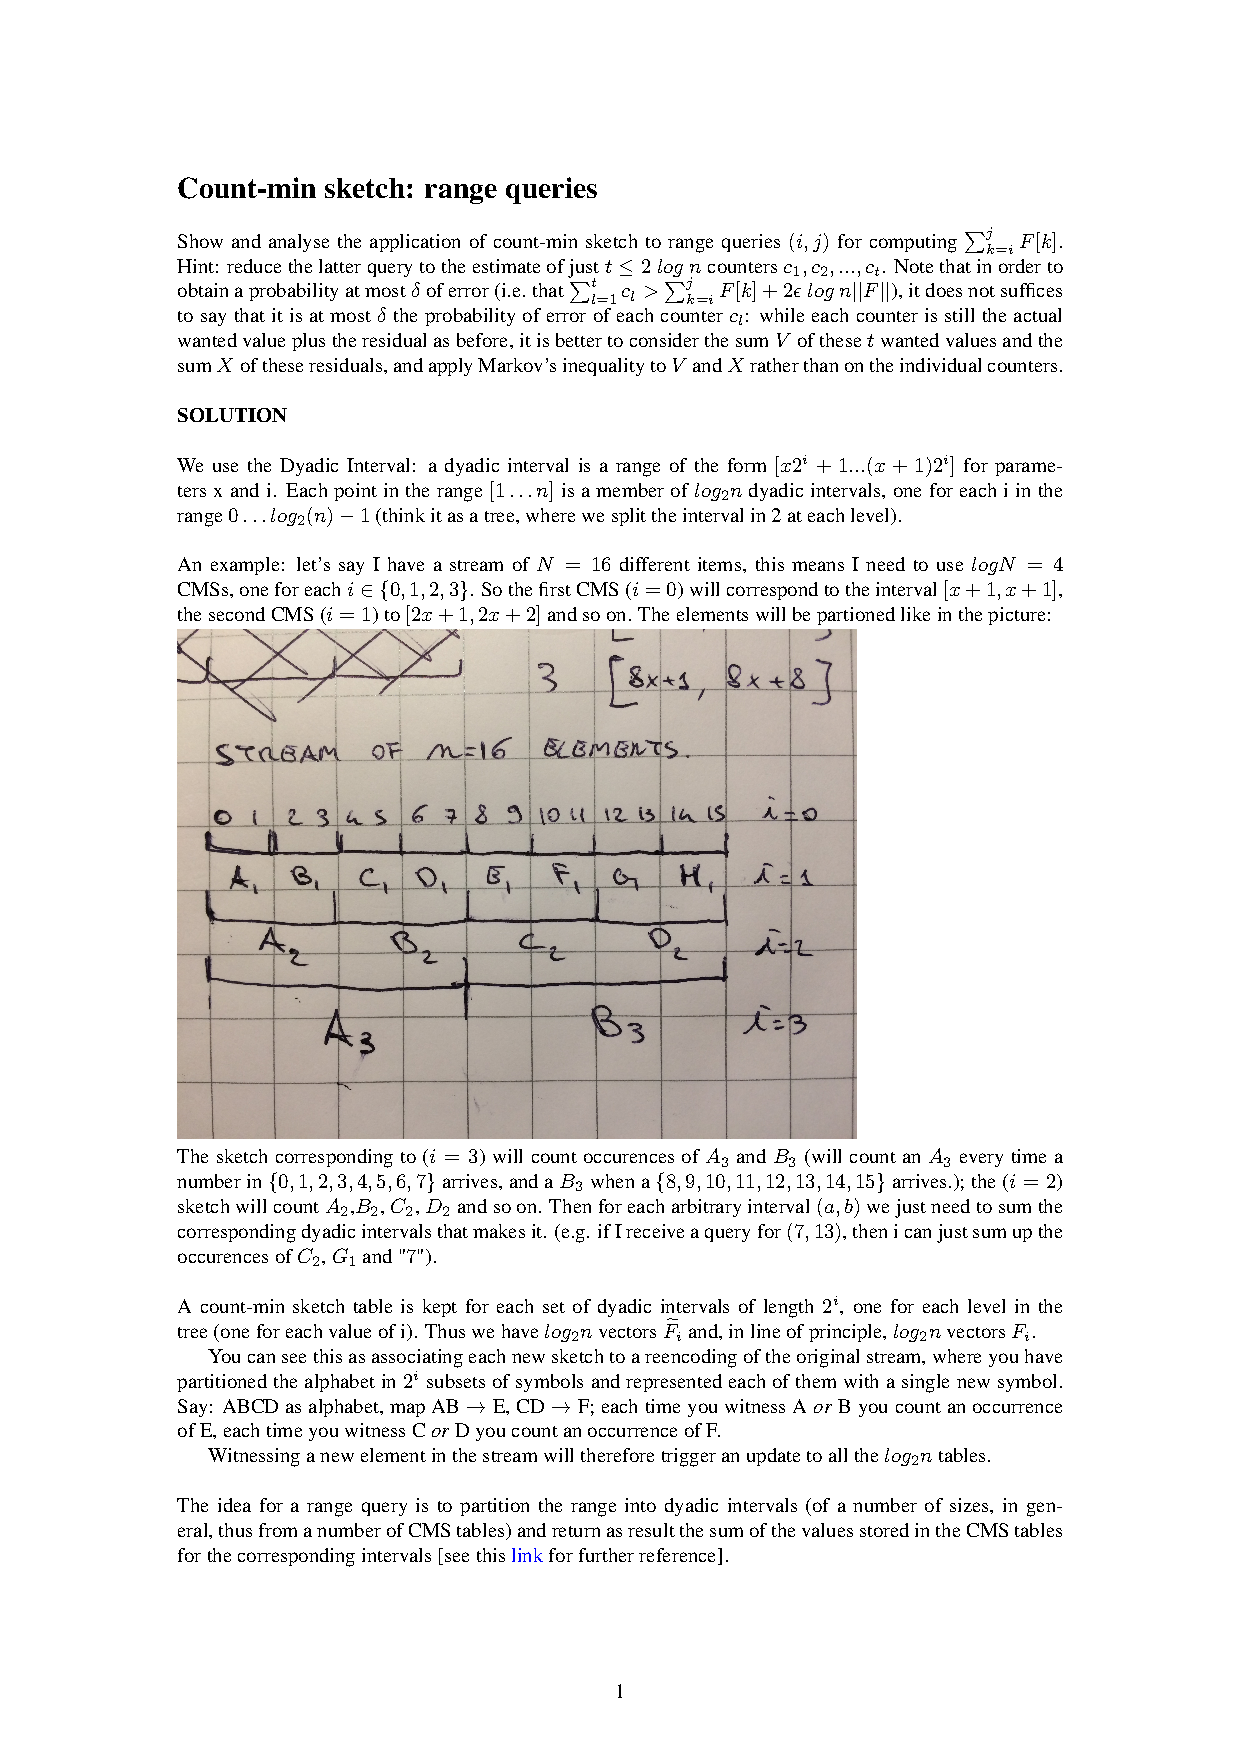
\includepdf[pages={1,2}]{../EX09/Problem9_SOLUTION}
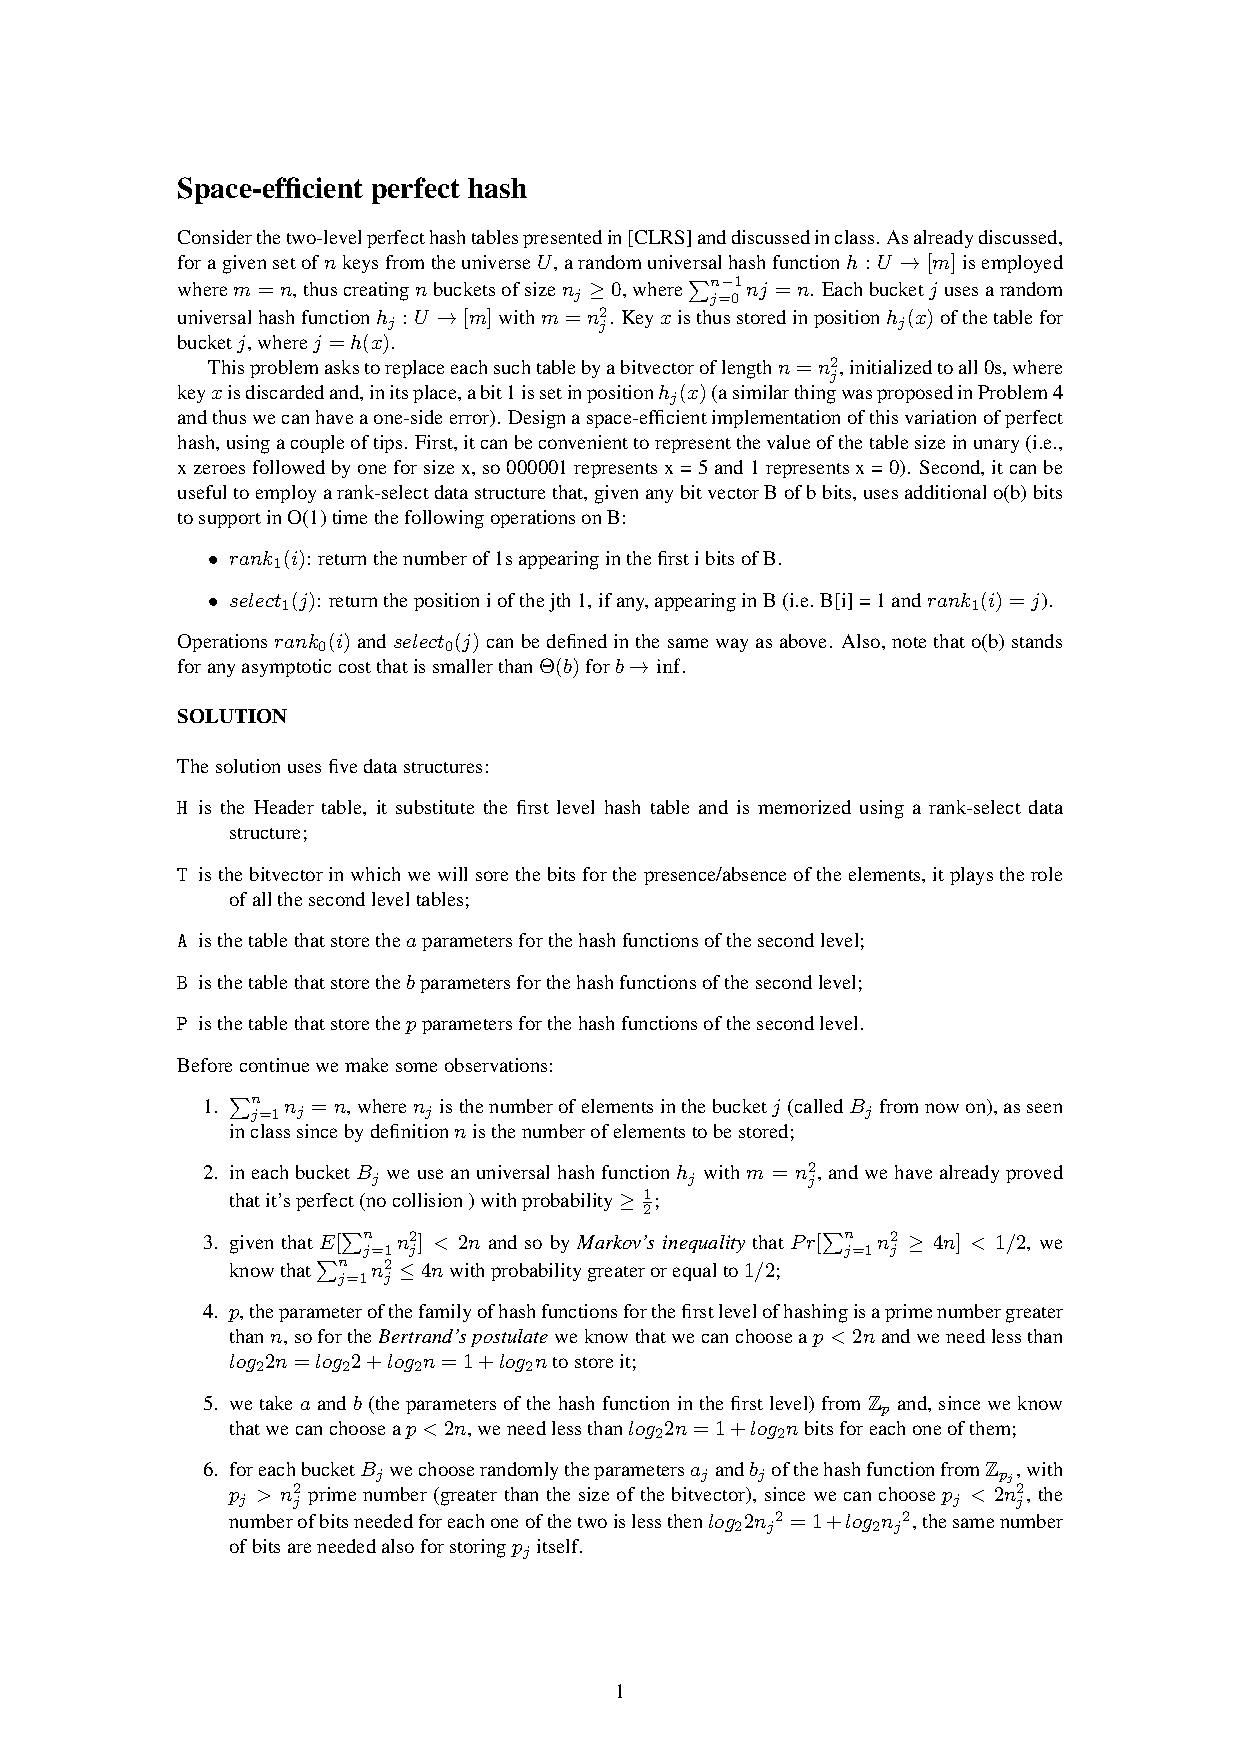
\includepdf[pages={1,2}]{../EX10/Problem10_SOLUTION}
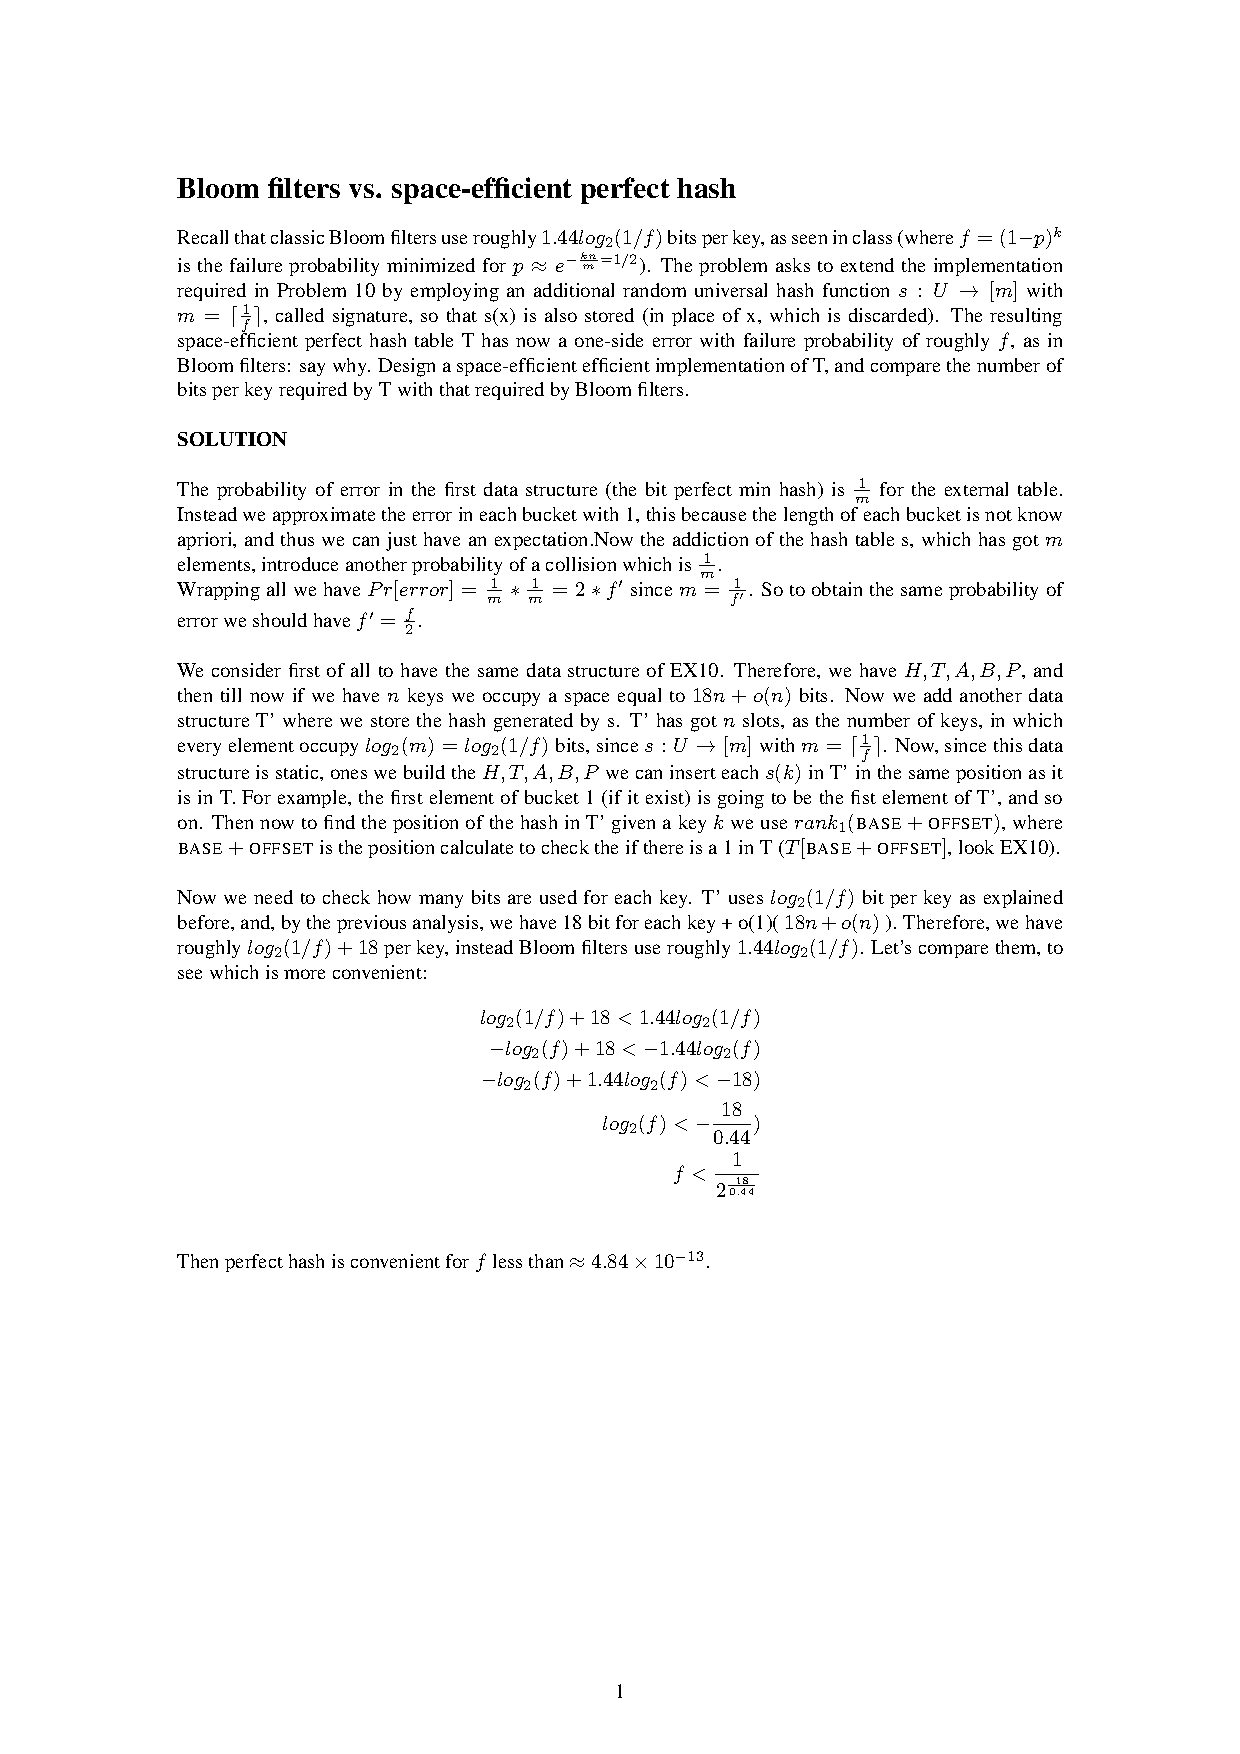
\includepdf[pages={1}]{../EX11/Problem11_SOLUTION}
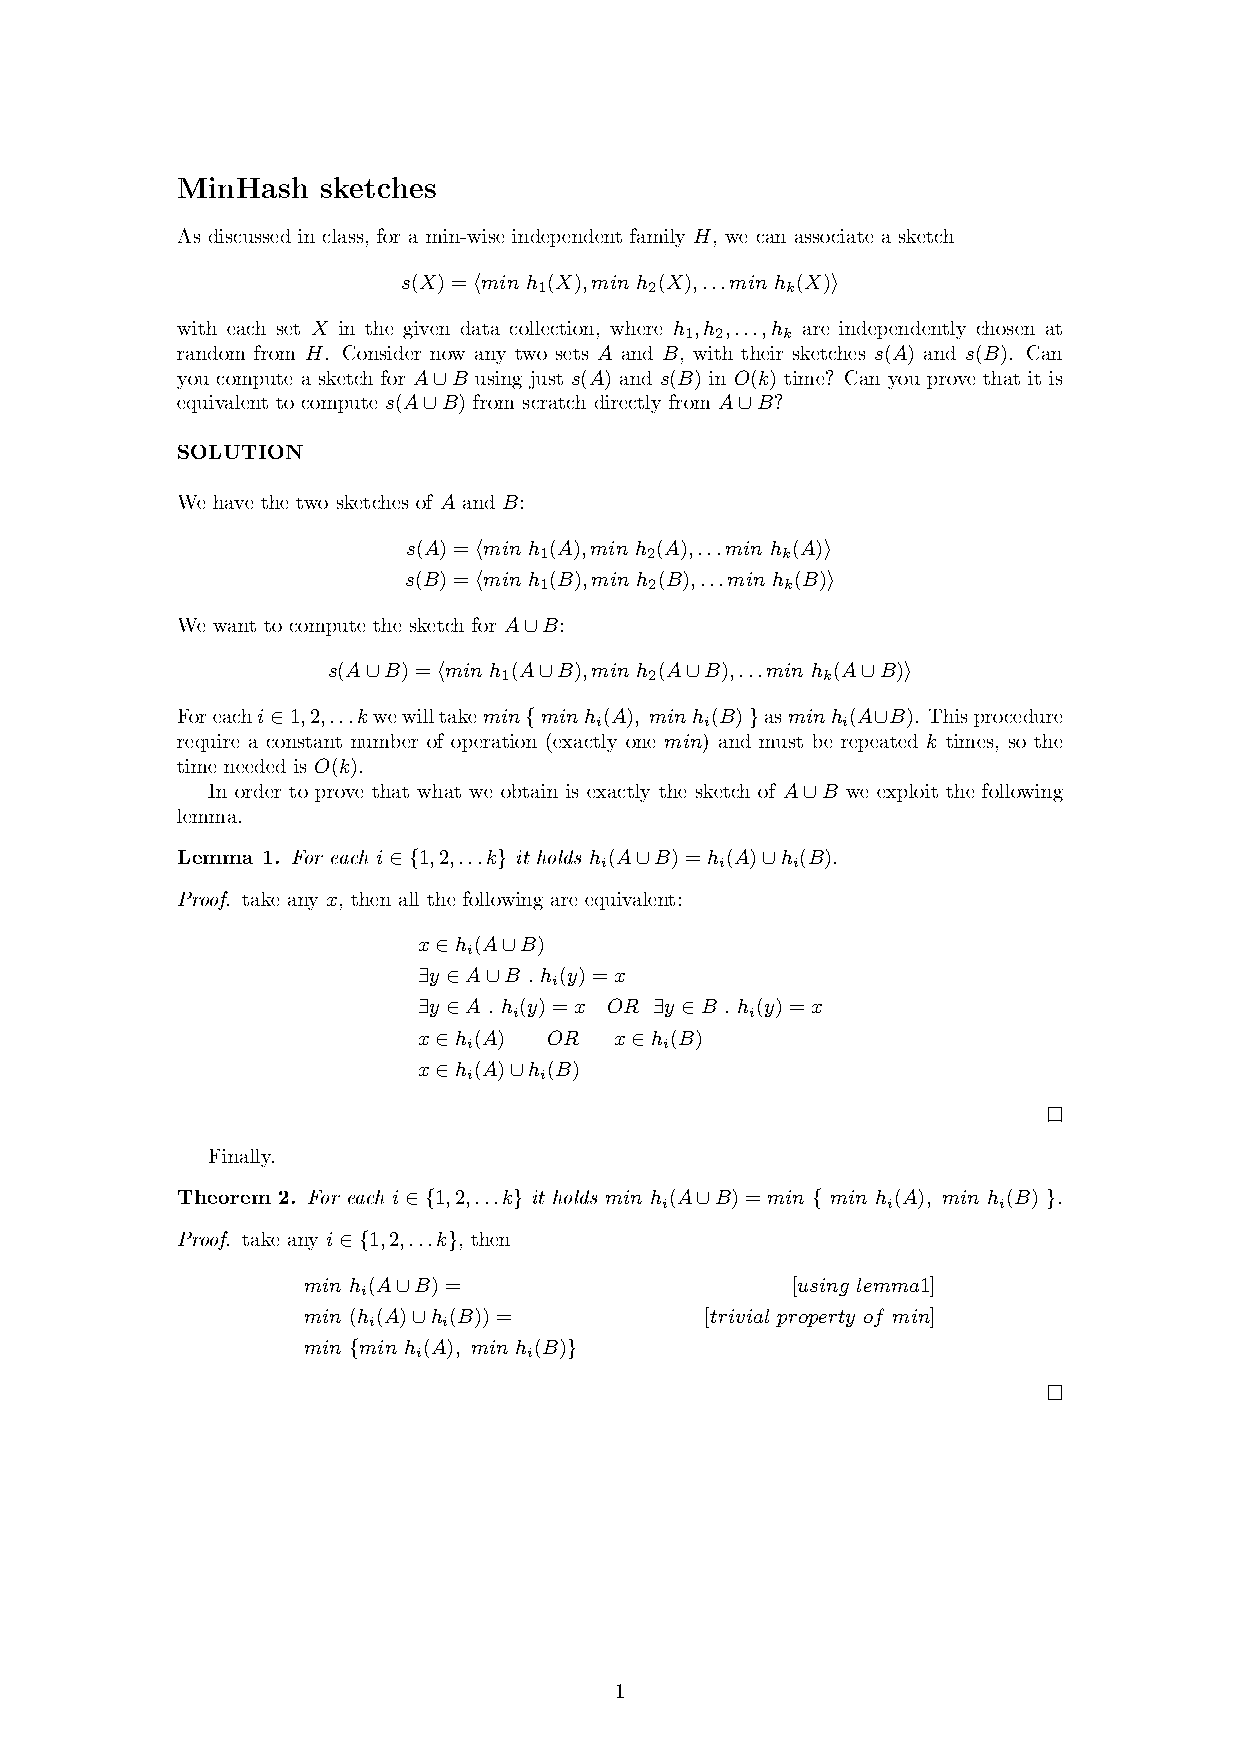
\includepdf[pages={1}]{../EX12/Problem12_SOLUTION}
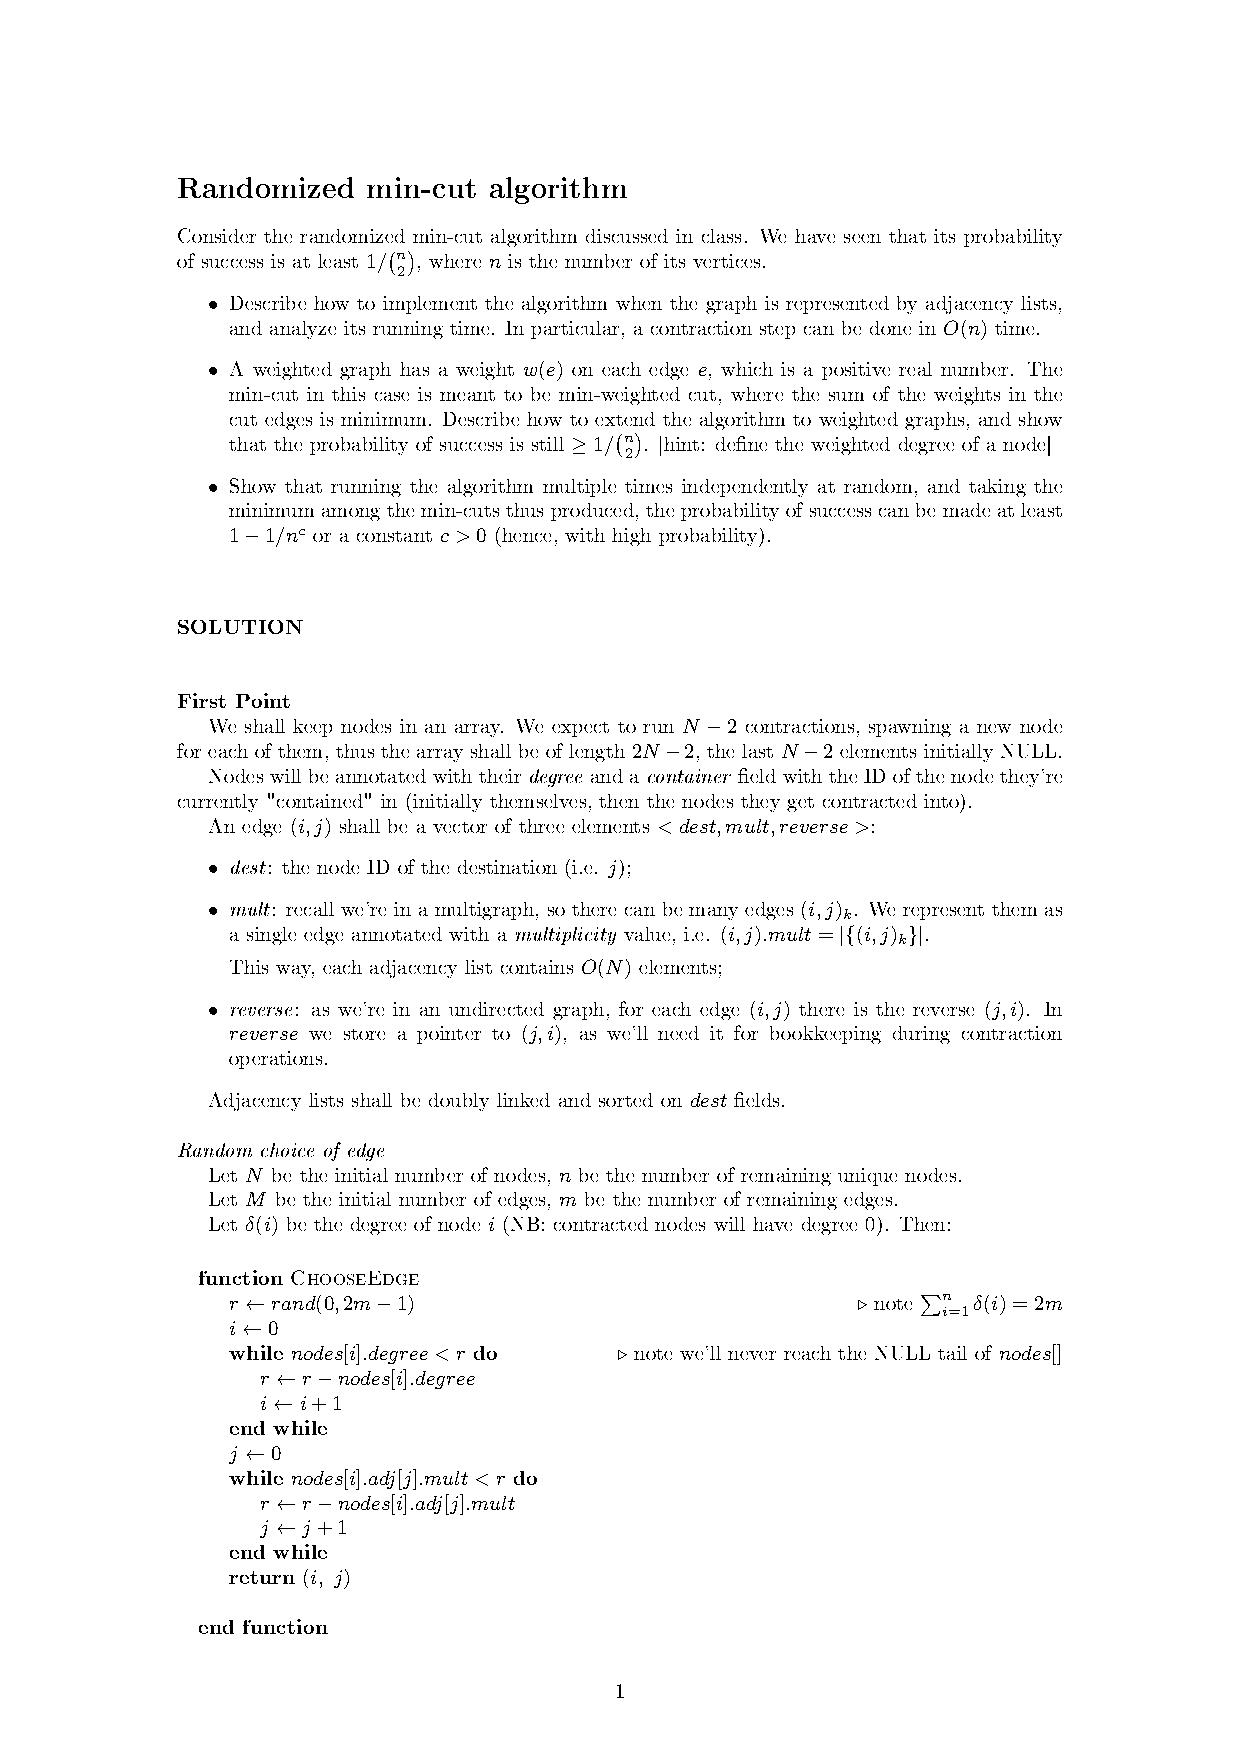
\includepdf[pages={1,2,3,4,5}]{../EX13/Problem13_SOLUTION}
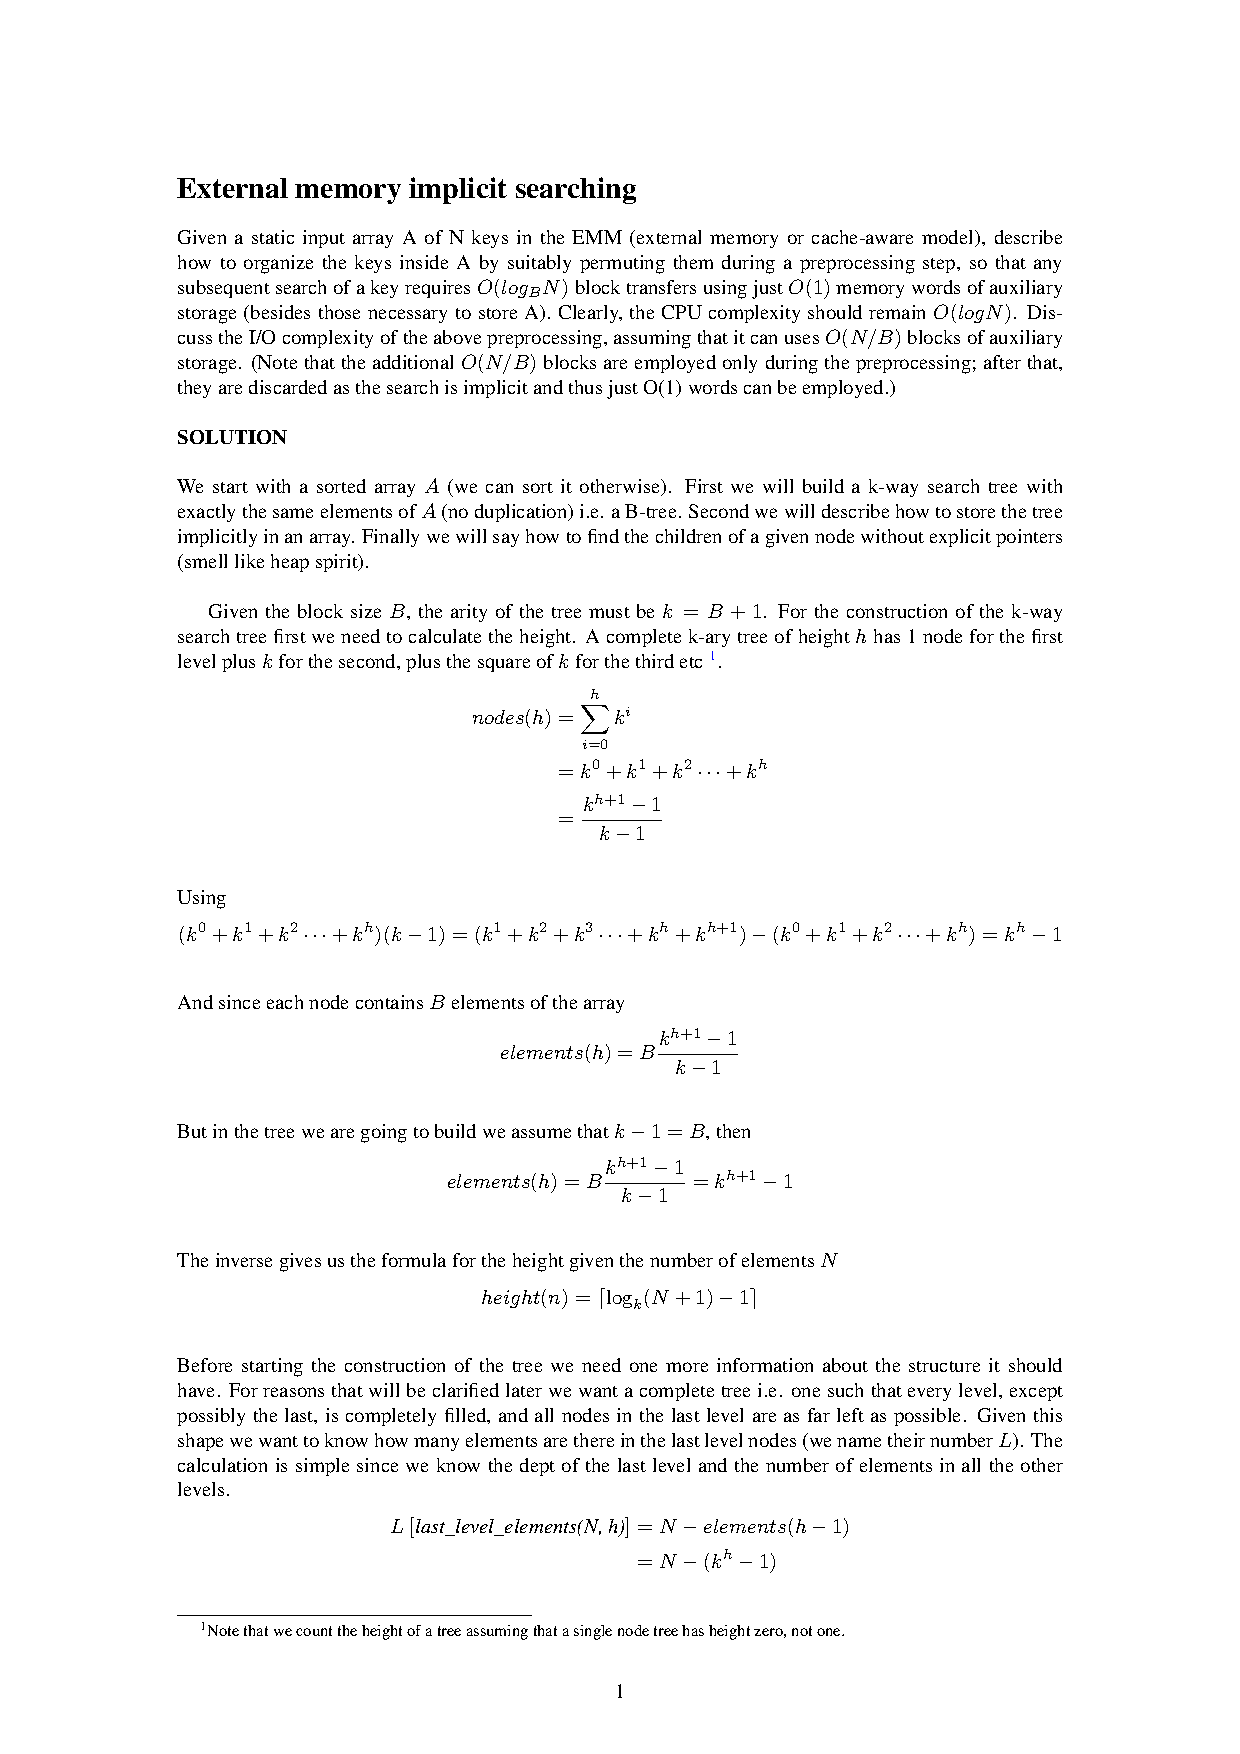
\includepdf[pages={1,2,3,4}]{../EX14/Problem14_SOLUTION}
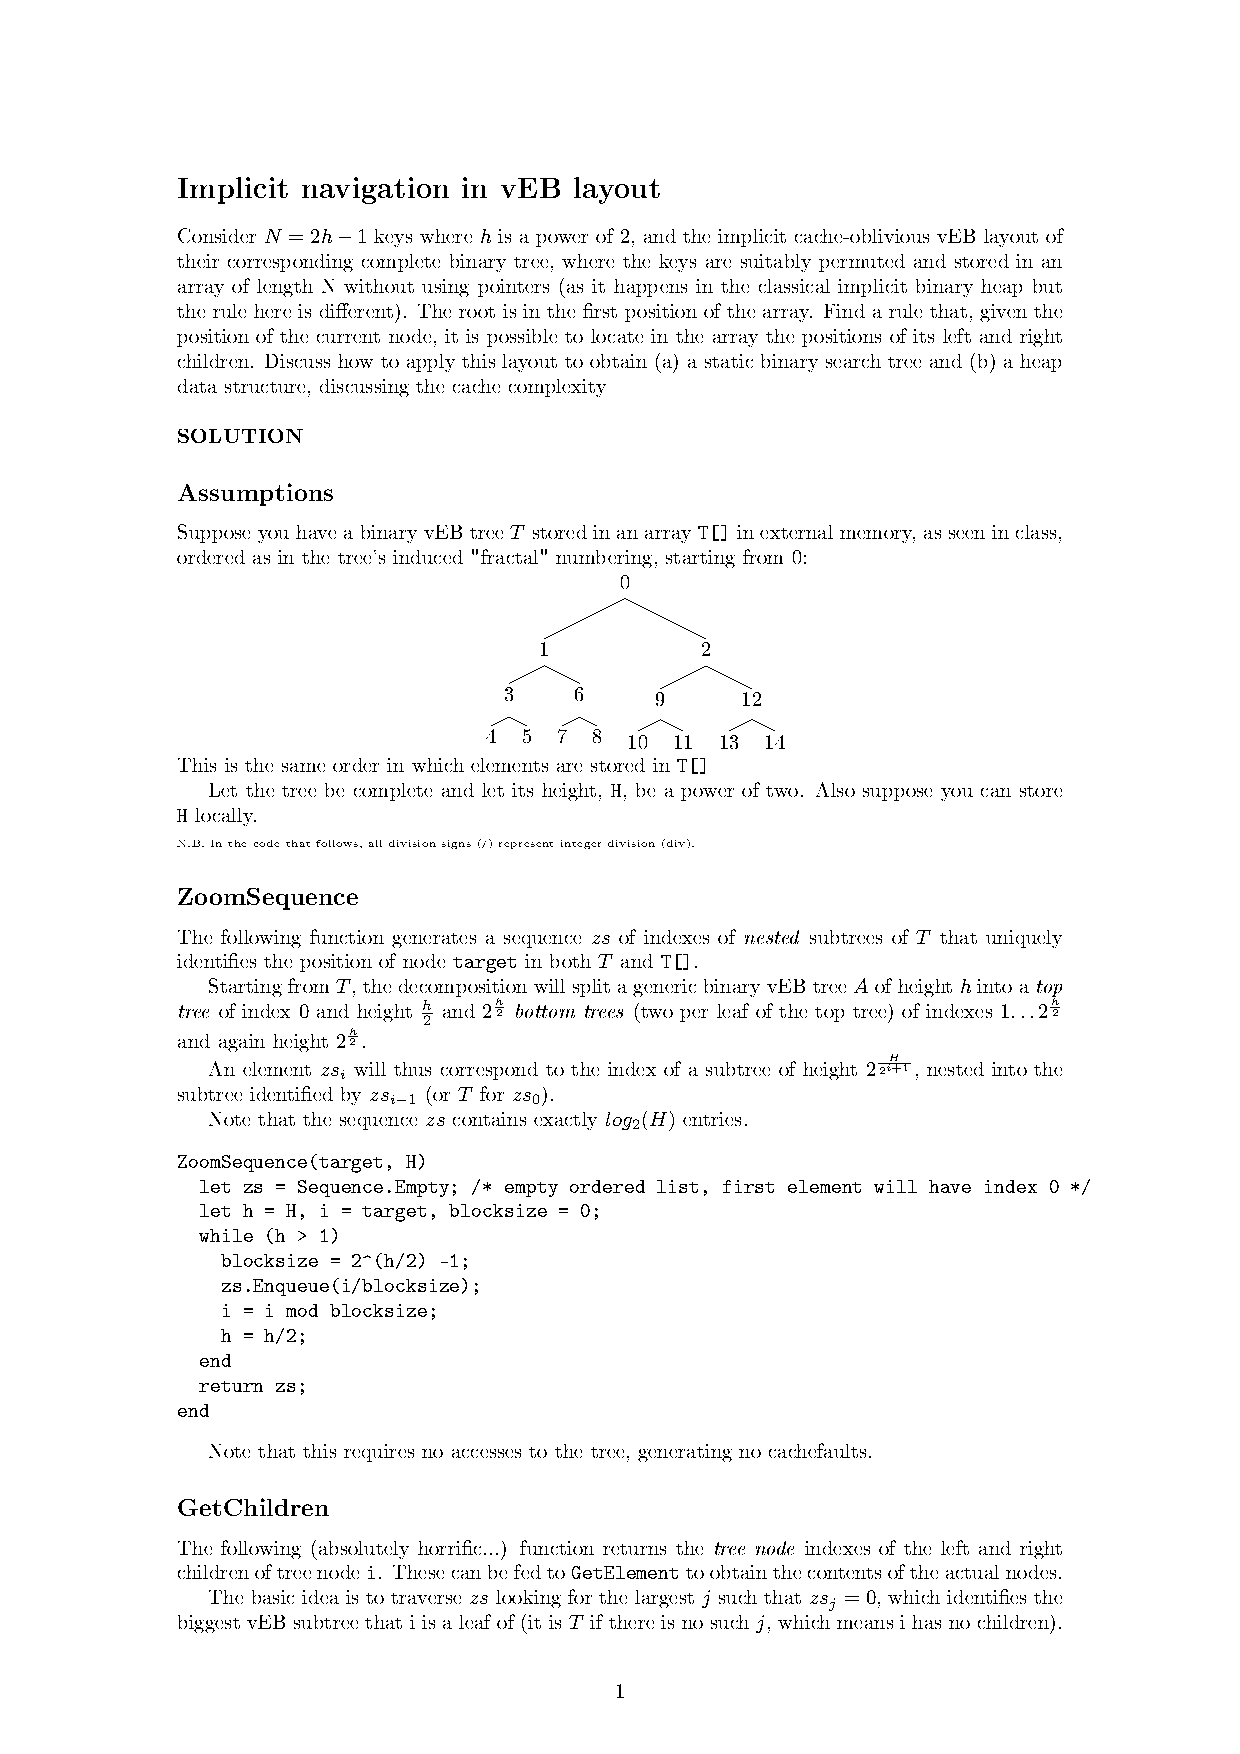
\includepdf[pages={1,2,3}]{../EX15/Problem15_SOLUTION}
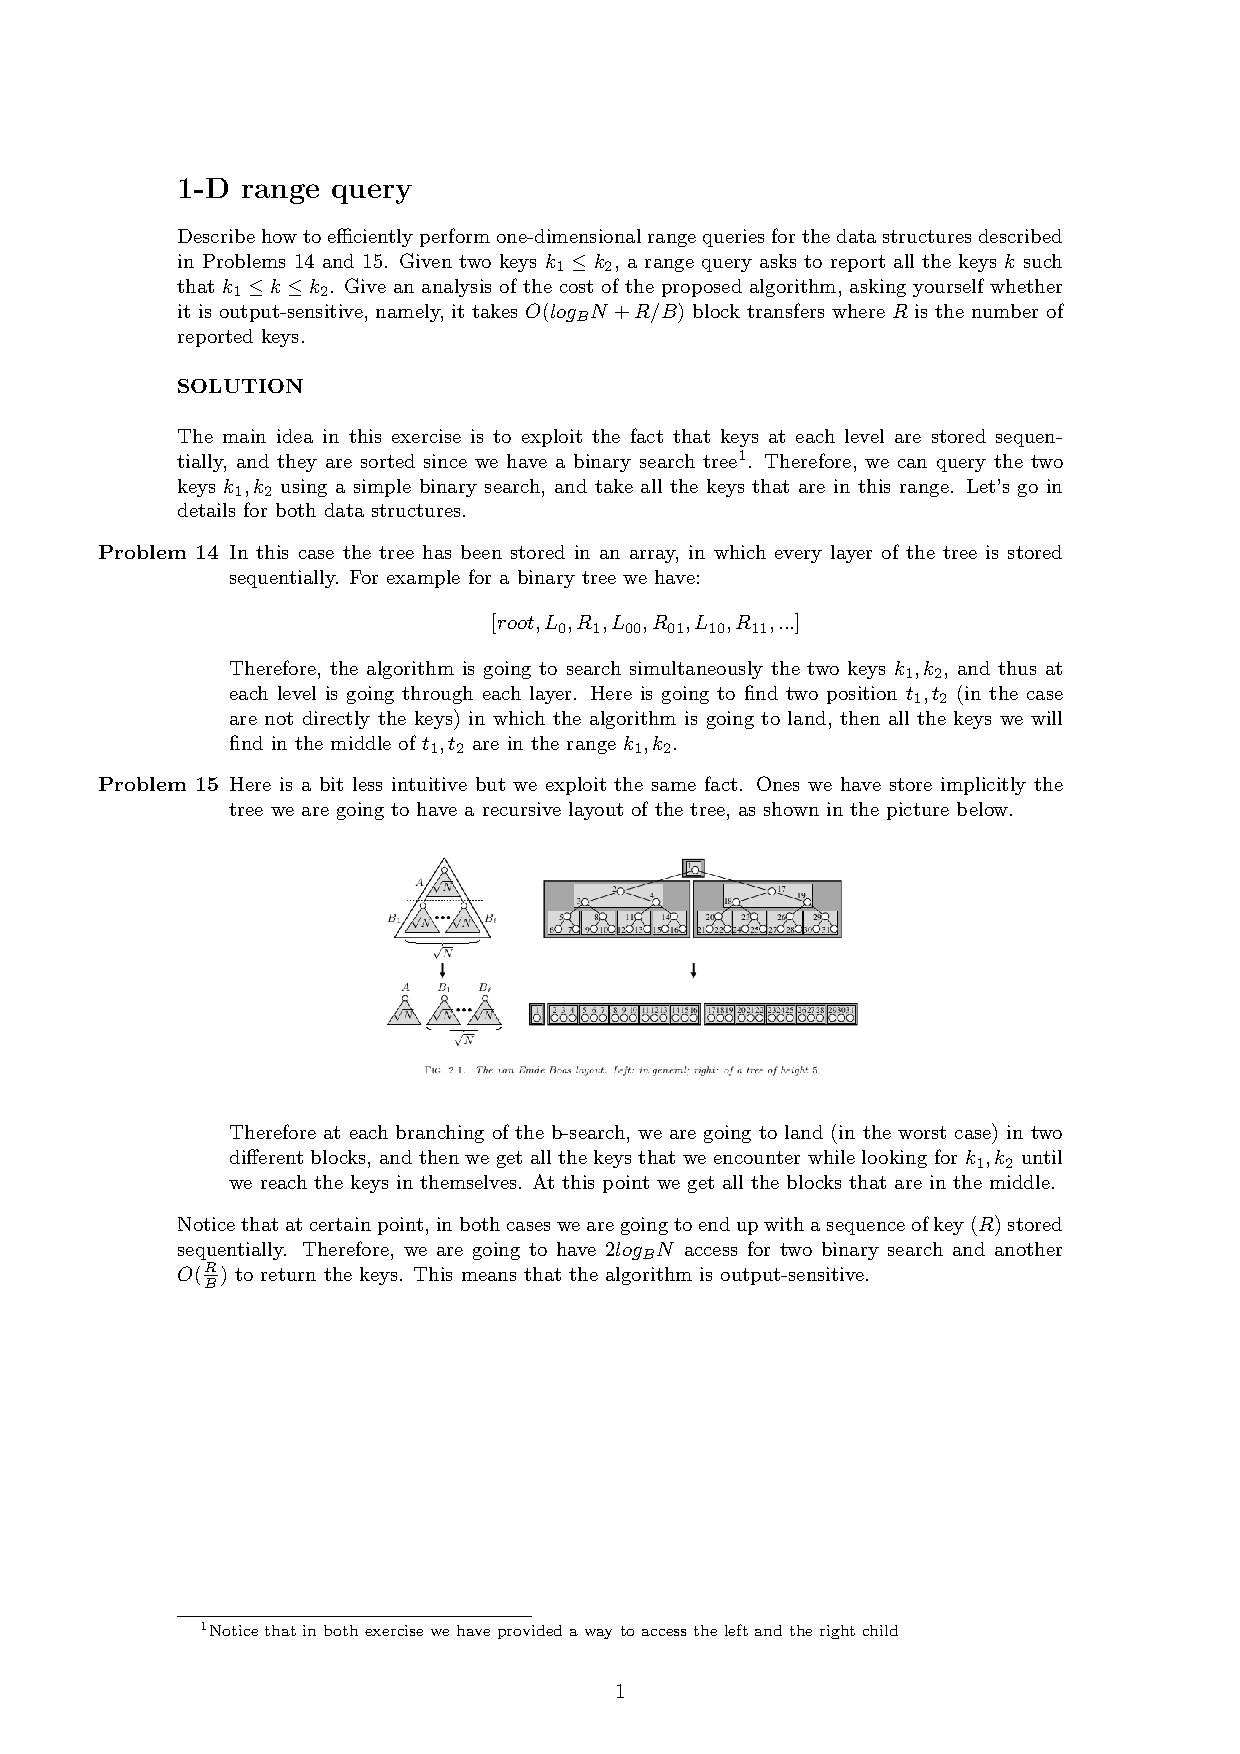
\includepdf[pages={1}]{../EX16/Problem16_SOLUTION}
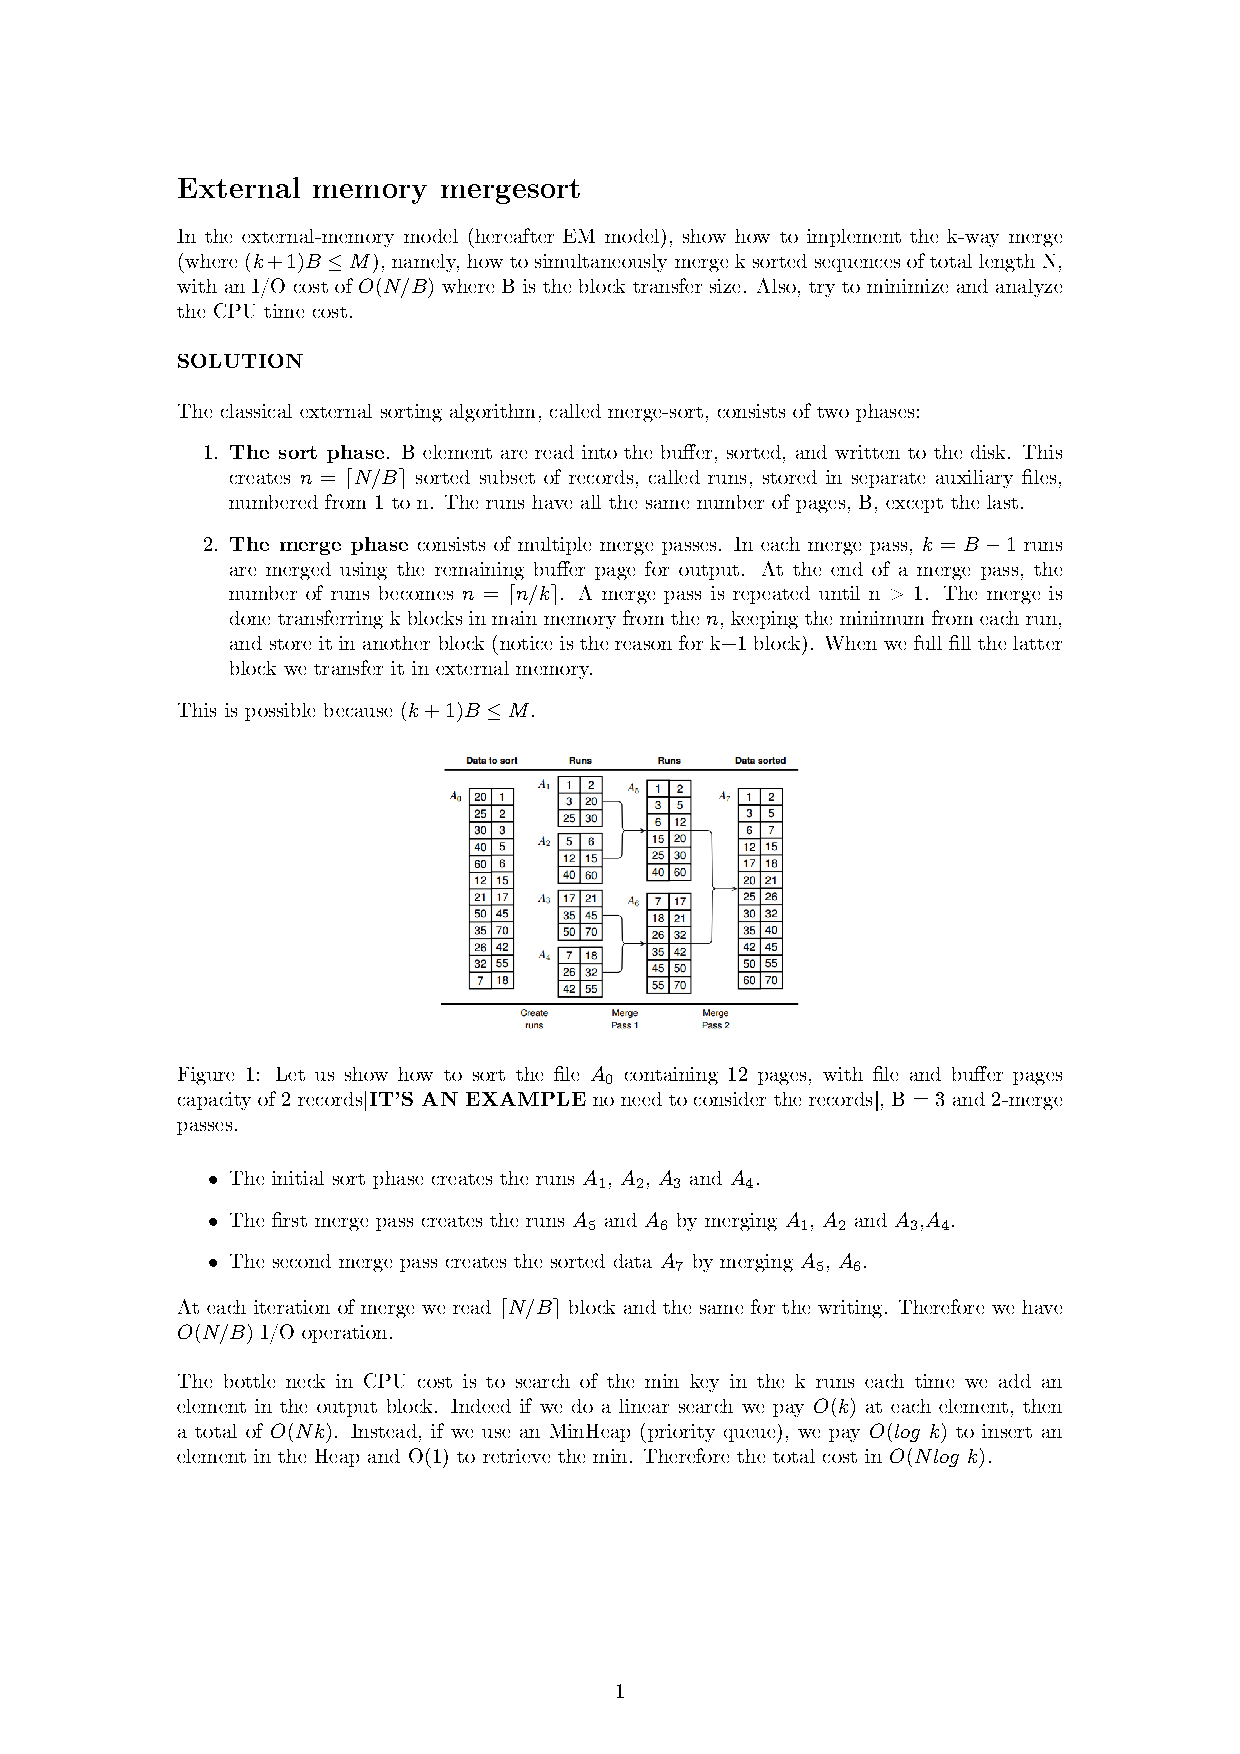
\includepdf[pages={1,2}]{../EX17/Problem17_SOLUTION}
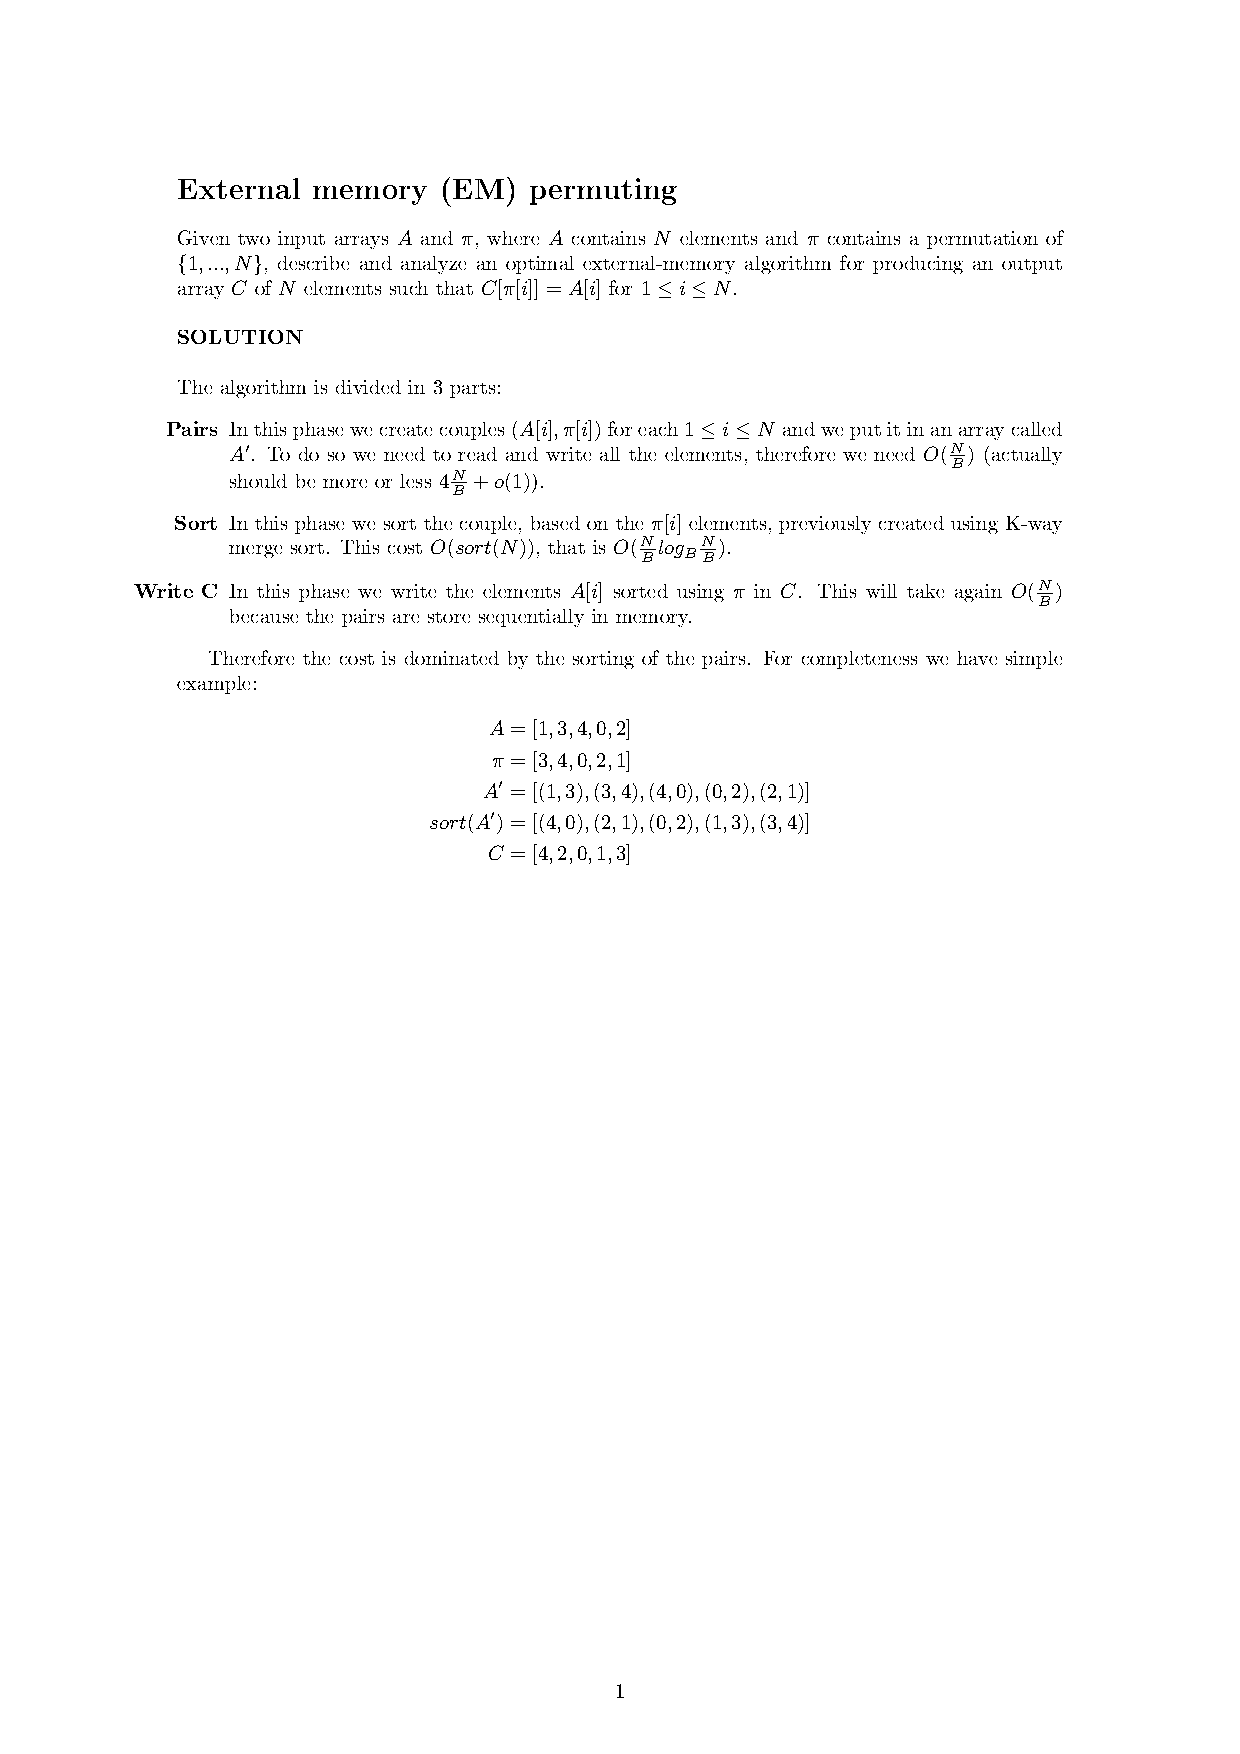
\includepdf[pages={1}]{../EX18/Problem18_SOLUTION}
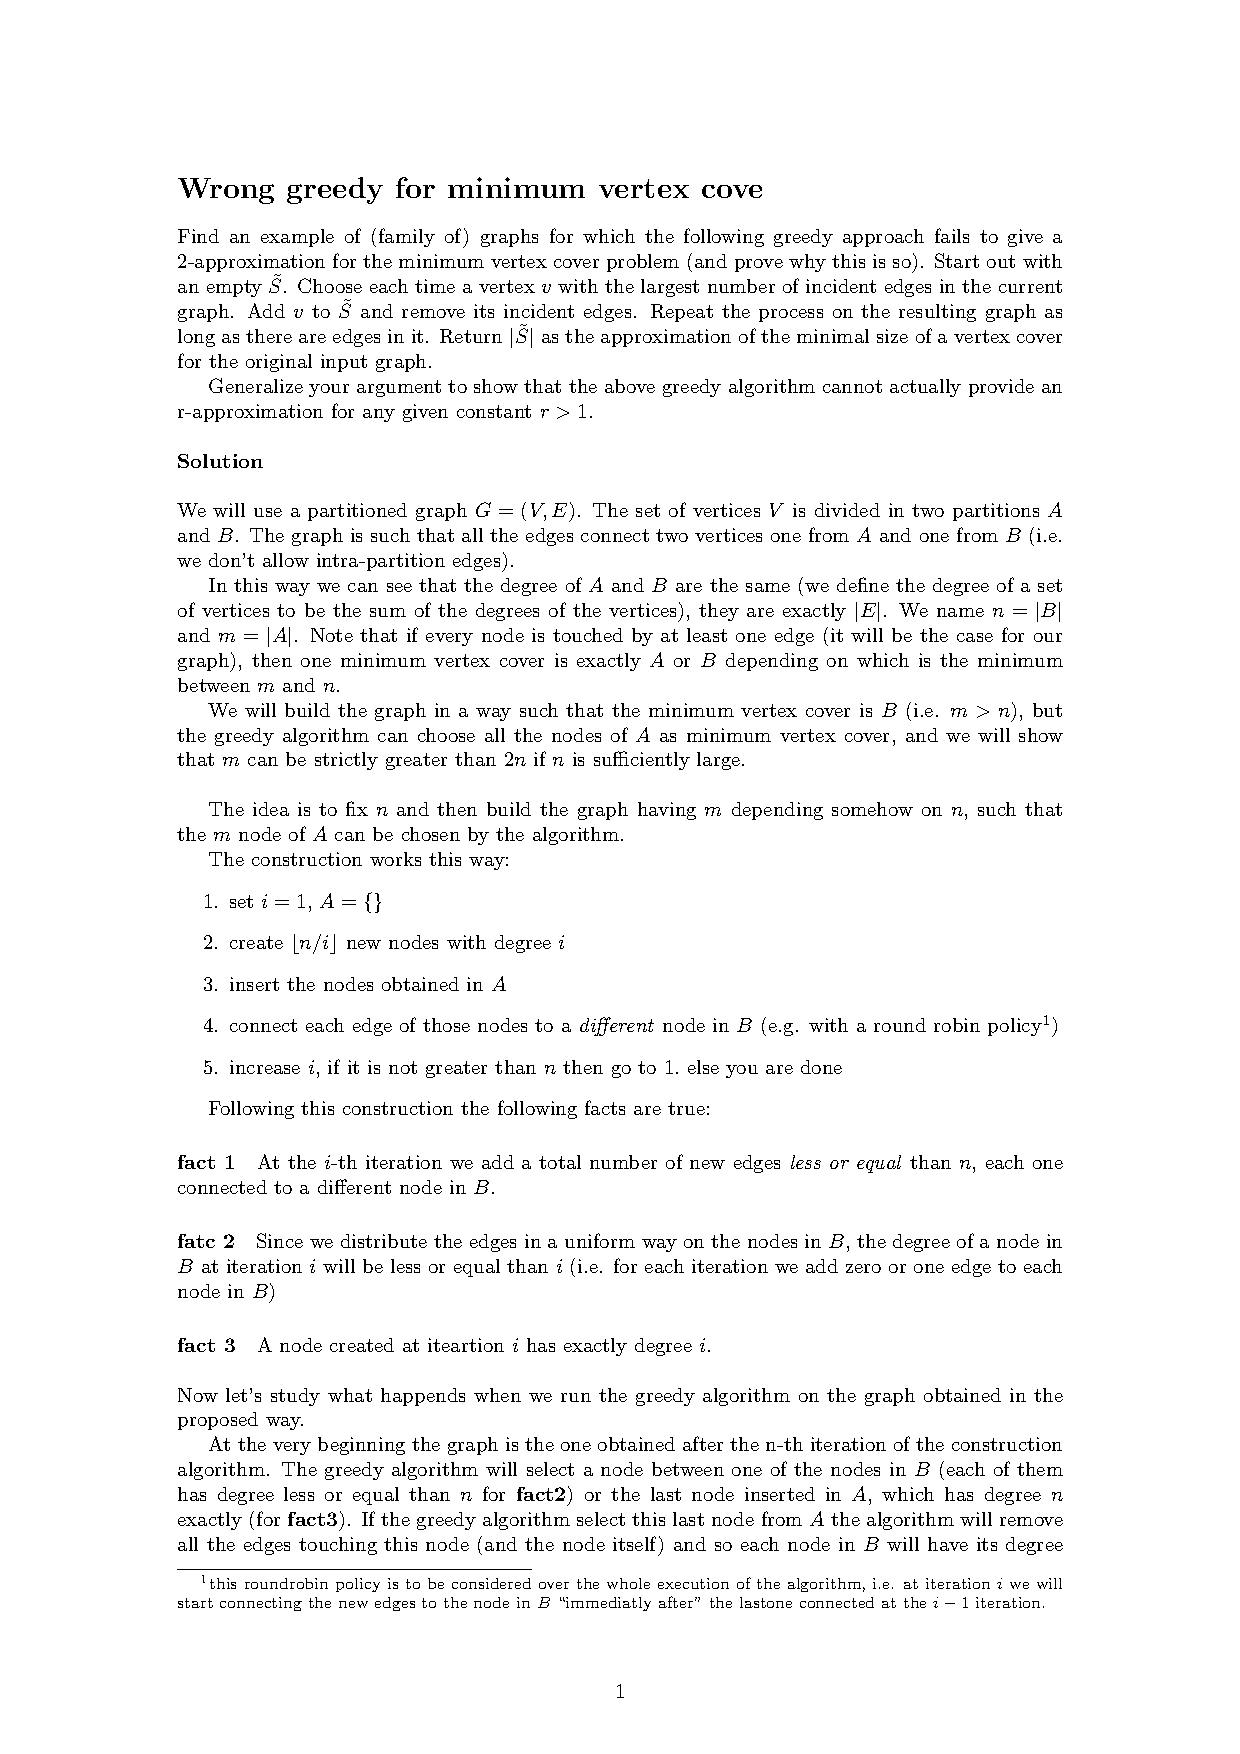
\includepdf[pages={1,2}]{../EX20/Problem20_SOLUTION}
\end{document}